% Options for packages loaded elsewhere
\PassOptionsToPackage{unicode}{hyperref}
\PassOptionsToPackage{hyphens}{url}
\PassOptionsToPackage{dvipsnames,svgnames,x11names}{xcolor}
%
\documentclass[
  11pt,
]{krantz}
\usepackage{amsmath,amssymb}
\usepackage{lmodern}
\usepackage{iftex}
\ifPDFTeX
  \usepackage[T1]{fontenc}
  \usepackage[utf8]{inputenc}
  \usepackage{textcomp} % provide euro and other symbols
\else % if luatex or xetex
  \usepackage{unicode-math}
  \defaultfontfeatures{Scale=MatchLowercase}
  \defaultfontfeatures[\rmfamily]{Ligatures=TeX,Scale=1}
  \setmonofont[Scale=0.775]{MesloLGS NF}
\fi
% Use upquote if available, for straight quotes in verbatim environments
\IfFileExists{upquote.sty}{\usepackage{upquote}}{}
\IfFileExists{microtype.sty}{% use microtype if available
  \usepackage[]{microtype}
  \UseMicrotypeSet[protrusion]{basicmath} % disable protrusion for tt fonts
}{}
\makeatletter
\@ifundefined{KOMAClassName}{% if non-KOMA class
  \IfFileExists{parskip.sty}{%
    \usepackage{parskip}
  }{% else
    \setlength{\parindent}{0pt}
    \setlength{\parskip}{6pt plus 2pt minus 1pt}}
}{% if KOMA class
  \KOMAoptions{parskip=half}}
\makeatother
\usepackage{xcolor}
\IfFileExists{xurl.sty}{\usepackage{xurl}}{} % add URL line breaks if available
\IfFileExists{bookmark.sty}{\usepackage{bookmark}}{\usepackage{hyperref}}
\hypersetup{
  pdftitle={Data Science per psicologi},
  pdfauthor={Corrado Caudek},
  colorlinks=true,
  linkcolor={Maroon},
  filecolor={Maroon},
  citecolor={Blue},
  urlcolor={Blue},
  pdfcreator={LaTeX via pandoc}}
\urlstyle{same} % disable monospaced font for URLs
\usepackage{color}
\usepackage{fancyvrb}
\newcommand{\VerbBar}{|}
\newcommand{\VERB}{\Verb[commandchars=\\\{\}]}
\DefineVerbatimEnvironment{Highlighting}{Verbatim}{commandchars=\\\{\}}
% Add ',fontsize=\small' for more characters per line
\usepackage{framed}
\definecolor{shadecolor}{RGB}{248,248,248}
\newenvironment{Shaded}{\begin{snugshade}}{\end{snugshade}}
\newcommand{\AlertTok}[1]{\textcolor[rgb]{0.33,0.33,0.33}{#1}}
\newcommand{\AnnotationTok}[1]{\textcolor[rgb]{0.37,0.37,0.37}{\textbf{\textit{#1}}}}
\newcommand{\AttributeTok}[1]{\textcolor[rgb]{0.61,0.61,0.61}{#1}}
\newcommand{\BaseNTok}[1]{\textcolor[rgb]{0.06,0.06,0.06}{#1}}
\newcommand{\BuiltInTok}[1]{#1}
\newcommand{\CharTok}[1]{\textcolor[rgb]{0.5,0.5,0.5}{#1}}
\newcommand{\CommentTok}[1]{\textcolor[rgb]{0.37,0.37,0.37}{\textit{#1}}}
\newcommand{\CommentVarTok}[1]{\textcolor[rgb]{0.37,0.37,0.37}{\textbf{\textit{#1}}}}
\newcommand{\ConstantTok}[1]{\textcolor[rgb]{0,0,0}{#1}}
\newcommand{\ControlFlowTok}[1]{\textcolor[rgb]{0.27,0.27,0.27}{\textbf{#1}}}
\newcommand{\DataTypeTok}[1]{\textcolor[rgb]{0.27,0.27,0.27}{#1}}
\newcommand{\DecValTok}[1]{\textcolor[rgb]{0.06,0.06,0.06}{#1}}
\newcommand{\DocumentationTok}[1]{\textcolor[rgb]{0.37,0.37,0.37}{\textbf{\textit{#1}}}}
\newcommand{\ErrorTok}[1]{\textcolor[rgb]{0.14,0.14,0.14}{\textbf{#1}}}
\newcommand{\ExtensionTok}[1]{#1}
\newcommand{\FloatTok}[1]{\textcolor[rgb]{0.06,0.06,0.06}{#1}}
\newcommand{\FunctionTok}[1]{\textcolor[rgb]{0,0,0}{#1}}
\newcommand{\ImportTok}[1]{#1}
\newcommand{\InformationTok}[1]{\textcolor[rgb]{0.37,0.37,0.37}{\textbf{\textit{#1}}}}
\newcommand{\KeywordTok}[1]{\textcolor[rgb]{0.27,0.27,0.27}{\textbf{#1}}}
\newcommand{\NormalTok}[1]{#1}
\newcommand{\OperatorTok}[1]{\textcolor[rgb]{0.43,0.43,0.43}{\textbf{#1}}}
\newcommand{\OtherTok}[1]{\textcolor[rgb]{0.37,0.37,0.37}{#1}}
\newcommand{\PreprocessorTok}[1]{\textcolor[rgb]{0.37,0.37,0.37}{\textit{#1}}}
\newcommand{\RegionMarkerTok}[1]{#1}
\newcommand{\SpecialCharTok}[1]{\textcolor[rgb]{0,0,0}{#1}}
\newcommand{\SpecialStringTok}[1]{\textcolor[rgb]{0.5,0.5,0.5}{#1}}
\newcommand{\StringTok}[1]{\textcolor[rgb]{0.5,0.5,0.5}{#1}}
\newcommand{\VariableTok}[1]{\textcolor[rgb]{0,0,0}{#1}}
\newcommand{\VerbatimStringTok}[1]{\textcolor[rgb]{0.5,0.5,0.5}{#1}}
\newcommand{\WarningTok}[1]{\textcolor[rgb]{0.37,0.37,0.37}{\textbf{\textit{#1}}}}
\usepackage{longtable,booktabs,array}
\usepackage{calc} % for calculating minipage widths
% Correct order of tables after \paragraph or \subparagraph
\usepackage{etoolbox}
\makeatletter
\patchcmd\longtable{\par}{\if@noskipsec\mbox{}\fi\par}{}{}
\makeatother
% Allow footnotes in longtable head/foot
\IfFileExists{footnotehyper.sty}{\usepackage{footnotehyper}}{\usepackage{footnote}}
\makesavenoteenv{longtable}
\usepackage{graphicx}
\makeatletter
\def\maxwidth{\ifdim\Gin@nat@width>\linewidth\linewidth\else\Gin@nat@width\fi}
\def\maxheight{\ifdim\Gin@nat@height>\textheight\textheight\else\Gin@nat@height\fi}
\makeatother
% Scale images if necessary, so that they will not overflow the page
% margins by default, and it is still possible to overwrite the defaults
% using explicit options in \includegraphics[width, height, ...]{}
\setkeys{Gin}{width=\maxwidth,height=\maxheight,keepaspectratio}
% Set default figure placement to htbp
\makeatletter
\def\fps@figure{htbp}
\makeatother
\setlength{\emergencystretch}{3em} % prevent overfull lines
\providecommand{\tightlist}{%
  \setlength{\itemsep}{0pt}\setlength{\parskip}{0pt}}
\setcounter{secnumdepth}{5}
\defaultfontfeatures{Scale=MatchLowercase}

\usepackage{booktabs}
\usepackage{longtable}
\usepackage[bf,singlelinecheck=off]{caption}

\usepackage{framed,color}
\definecolor{shadecolor}{RGB}{248,248,248}

\renewcommand{\textfraction}{0.05}
\renewcommand{\topfraction}{0.8}
\renewcommand{\bottomfraction}{0.8}
\renewcommand{\floatpagefraction}{0.75}

\renewenvironment{quote}{\begin{VF}}{\end{VF}}
\let\oldhref\href
\renewcommand{\href}[2]{#2\footnote{\url{#1}}}

\ifxetex
  \usepackage{letltxmacro}
  \setlength{\XeTeXLinkMargin}{1pt}
  \LetLtxMacro\SavedIncludeGraphics\includegraphics
  \def\includegraphics#1#{% #1 catches optional stuff (star/opt. arg.)
    \IncludeGraphicsAux{#1}%
  }%
  \newcommand*{\IncludeGraphicsAux}[2]{%
    \XeTeXLinkBox{%
      \SavedIncludeGraphics#1{#2}%
    }%
  }%
\fi

\makeatletter
\newenvironment{kframe}{%
\medskip{}
\setlength{\fboxsep}{.8em}
 \def\at@end@of@kframe{}%
 \ifinner\ifhmode%
  \def\at@end@of@kframe{\end{minipage}}%
  \begin{minipage}{\columnwidth}%
 \fi\fi%
 \def\FrameCommand##1{\hskip\@totalleftmargin \hskip-\fboxsep
 \colorbox{shadecolor}{##1}\hskip-\fboxsep
     % There is no \\@totalrightmargin, so:
     \hskip-\linewidth \hskip-\@totalleftmargin \hskip\columnwidth}%
 \MakeFramed {\advance\hsize-\width
   \@totalleftmargin\z@ \linewidth\hsize
   \@setminipage}}%
 {\par\unskip\endMakeFramed%
 \at@end@of@kframe}
\makeatother

\renewenvironment{Shaded}{\begin{kframe}}{\end{kframe}}

\usepackage{makeidx}
\makeindex

\urlstyle{tt}

\usepackage{amsthm}
\makeatletter
\def\thm@space@setup{%
  \thm@preskip=8pt plus 2pt minus 4pt
  \thm@postskip=\thm@preskip
}
\makeatother

\newcommand{\E}{\mathbb{E}} % Define expected value operator
\DeclareMathOperator{\Var}{\mathbb{V}} % Define variance operator
\DeclareMathOperator{\SD}{SD} % Define sd operator
\DeclareMathOperator{\Cov}{Cov} % Define covariance operator
\DeclareMathOperator{\Corr}{Corr} % Define correlation operator
\DeclareMathOperator{\Me}{Me} % Define mediane operator
\DeclareMathOperator{\Mo}{Mo} % Define mode operator
\DeclareMathOperator{\Bin}{Bin} % Define binomial operator
\DeclareMathOperator{\Bernoulli}{Bernoulli} % Define Bernoulli operator
\DeclareMathOperator{\Poi}{Poi} % Define Poisson operator
\DeclareMathOperator{\Uniform}{Uniform} % Define Uniform operator
\DeclareMathOperator{\Cauchy}{Cauchy} % Define Cauchy operator
\DeclareMathOperator{\elpd}{elpd} % Define elpd operator
\DeclareMathOperator{\lppd}{lppd} % Define lppd operator
\DeclareMathOperator{\LOO}{LOO} % Define LOO operator
\DeclareMathOperator{\Ber}{\mathscr{B}} % Define Bernoulli operator
\DeclareMathOperator{\B}{B} % beta function
% \mbox{B}(a, b) % beta function
% \mbox{Beta}(a, b) % beta distribution
\newcommand{\R}{\textsf{R}} % Define R programming language symbol
\newcommand{\Real}{\mathbb{R}} % Define real number operator
\newcommand{\Prob}{\mathscr{P}}
\DeclareMathOperator{\argmin}{arg\,min} % thin space, limits on side in displays
\DeclareMathOperator{\argmax}{arg\,max} % no space, limits on side in displays

\raggedbottom % allow variable (ragged) site heights
\frenchspacing

\usepackage[
 labelfont=bf,
 font={small, it}
]{caption}
\usepackage{upquote} % print correct quotes in verbatim-environments
\usepackage{empheq}
\usepackage{xfrac}

\usepackage{polyglossia}
\setmainlanguage{italian}

% \DeclareMathSizes{10}{9}{7}{5}

\frontmatter
\ifLuaTeX
  \usepackage{selnolig}  % disable illegal ligatures
\fi
\usepackage[]{natbib}
\bibliographystyle{apalike}

\title{Data Science per psicologi}
\author{Corrado Caudek}
\date{2022-01-18}

\usepackage{amsthm}
\newtheorem{theorem}{Teorema}[chapter]
\newtheorem{lemma}{Lemma}[chapter]
\newtheorem{corollary}{Corollario}[chapter]
\newtheorem{proposition}{Proposizione}[chapter]
\newtheorem{conjecture}{Congettura}[chapter]
\theoremstyle{definition}
\newtheorem{definition}{Definizione}[chapter]
\theoremstyle{definition}
\newtheorem{example}{Esempio}[chapter]
\theoremstyle{definition}
\newtheorem{exercise}{Esercizio}[chapter]
\theoremstyle{definition}
\newtheorem{hypothesis}{Hypothesis}[chapter]
\theoremstyle{remark}
\newtheorem*{remark}{Osservazione}
\newtheorem*{solution}{Soluzione}
\begin{document}
\maketitle

\cleardoublepage\newpage\thispagestyle{empty}\null
% \cleardoublepage\newpage\thispagestyle{empty}\null
%\cleardoublepage\newpage
\thispagestyle{empty}
\begin{center}
\Large{Psicometria -- AA 2021/2022}

\vskip20pt

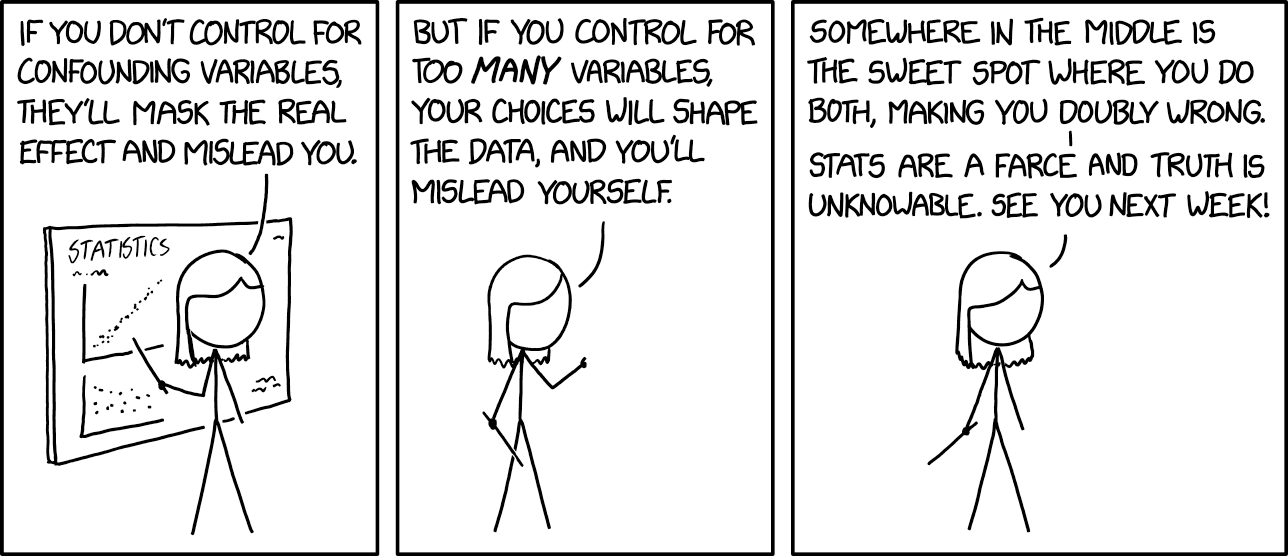
\includegraphics{images/confounding_variables.png}
\end{center}

\setlength{\abovedisplayskip}{-5pt}
\setlength{\abovedisplayshortskip}{-5pt}

{
\hypersetup{linkcolor=}
\setcounter{tocdepth}{2}
\tableofcontents
}
\listoffigures
\listoftables
\hypertarget{prefazione}{%
\chapter*{Prefazione}\label{prefazione}}


\emph{Data Science per psicologi} contiene il materiale delle lezioni dell'insegnamento di \emph{Psicometria B000286} (A.A. 2021/2022) rivolto agli studenti del primo anno del Corso di Laurea in Scienze e Tecniche Psicologiche dell'Università degli Studi di Firenze. \emph{Psicometria} si propone di fornire agli studenti un'introduzione all'analisi dei dati in psicologia. Le conoscenze/competenze che verranno sviluppate in questo insegnamento sono quelle della Data science, ovvero un insieme di conoscenze/competenze che si pongono all'intersezione tra statistica (ovvero, richiedono la capacità di comprendere teoremi statistici) e informatica (ovvero, richiedono la capacità di sapere utilizzare un software).

\hypertarget{la-psicologia-e-la-data-science}{%
\section*{La psicologia e la Data science}\label{la-psicologia-e-la-data-science}}


Sembra sensato spendere due parole su un tema che è importante per gli studenti: quello indicato dal titolo di questo Capitolo. È ovvio che agli studenti di psicologia la statistica non piace. Se piacesse, forse studierebbero Data science e non psicologia; ma non lo fanno. Di conseguenza, gli studenti di psicologia si chiedono: ``perché dobbiamo perdere tanto tempo a studiare queste cose quando in realtà quello che ci interessa è tutt'altro?'' Questa è una bella domanda.

C'è una ragione molto semplice che dovrebbe farci capire perché la Data science è così importante per la psicologia. Infatti, a ben pensarci, la psicologia è una disciplina intrinsecamente statistica, se per statistica intendiamo quella disciplina che studia la variazione delle caratteristiche degli individui nella popolazione. La psicologia studia \emph{gli individui} ed è proprio la variabilità inter- e intra-individuale ciò che vogliamo descrivere e, in certi casi, predire. In questo senso, la psicologia è molto diversa dall'ingegneria, per esempio. Le proprietà di un determinato ponte sotto certe condizioni, ad esempio, sono molto simili a quelle di un altro ponte, sotto le medesime condizioni. Quindi, per un ingegnere la statistica è poco importante: le proprietà dei materiali sono unicamente dipendenti dalla loro composizione e restano costanti. Ma lo stesso non può dirsi degli individui: ogni individuo è unico e cambia nel tempo. E le variazioni tra gli individui, e di un individuo nel tempo, sono l'oggetto di studio proprio della psicologia: è dunque chiaro che i problemi che la psicologia si pone sono molto diversi da quelli affrontati, per esempio, dagli ingegneri. Questa è la ragione per cui abbiamo tanto bisogno della Data science in psicologia: perché la Data science ci consente di descrivere la variazione e il cambiamento. E queste sono appunto le caratteristiche di base dei fenomeni psicologici.

Sono sicuro che, leggendo queste righe, a molti studenti sarà venuta in mente la seguente domanda: perché non chiediamo a qualche esperto di fare il ``lavoro sporco'' (ovvero le analisi statistiche) per noi, mentre noi (gli psicologi) ci occupiamo solo di ciò che ci interessa, ovvero dei problemi psicologici slegati dai dettagli ``tecnici'' della Data science? La risposta a questa domanda è che non è possibile progettare uno studio psicologico sensato senza avere almeno una comprensione rudimentale della Data science. Le tematiche della Data science non possono essere ignorate né dai ricercatori in psicologia né da coloro che svolgono la professione di psicologo al di fuori dell'Università. Infatti, anche i professionisti al di fuori dall'università non possono fare a meno di leggere la letteratura psicologica più recente: il continuo aggiornamento delle conoscenze è infatti richiesto dalla deontologia della professione. Ma per potere fare questo è necessario conoscere un bel po' di Data science! Basta aprire a caso una rivista specialistica di psicologia per rendersi conto di quanto ciò sia vero: gli articoli che riportano i risultati delle ricerche psicologiche sono zeppi di analisi statistiche e di modelli formali. E la comprensione della letteratura psicologica rappresenta un requisito minimo nel bagaglio professionale dello psicologo.

Le considerazioni precedenti cercano di chiarire il seguente punto: la Data science non è qualcosa da studiare a malincuore, in un singolo insegnamento universitario, per poi poterla tranquillamente dimenticare. Nel bene e nel male, gli psicologi usano gli strumenti della Data science in tantissimi ambiti della loro attività professionale: in particolare quando costruiscono, somministrano e interpretano i test psicometrici. È dunque chiaro che possedere delle solide basi di Data science è un tassello imprescindibile del bagaglio professionale dello psicologo. In questo insegnamento verrano trattati i temi base della Data science e verrà adottato un punto di vista bayesiano, che corrisponde all'approccio più recente e sempre più diffuso in psicologia.

\hypertarget{come-studiare}{%
\section*{Come studiare}\label{come-studiare}}


Il giusto metodo di studio per prepararsi all'esame di Psicometria è quello di seguire attivamente le lezioni, assimilare i concetti via via che essi vengono presentati e verificare in autonomia le procedure presentate a lezione. Incoraggio gli studenti a farmi domande per chiarire ciò che non è stato capito appieno. Incoraggio gli studenti a utilizzare i forum attivi su Moodle e, soprattutto, a svolgere gli esercizi proposti su Moodle. I problemi forniti su Moodle rappresentano il livello di difficoltà richiesto per superare l'esame e consentono allo studente di comprendere se le competenze sviluppate fino a quel punto sono sufficienti rispetto alle richieste dell'esame.

La prima fase dello studio, che è sicuramente individuale, è quella in cui è necessario acquisire le conoscenze teoriche relative ai problemi che saranno presentati all'esame. La seconda fase di studio, che può essere facilitata da scambi con altri e da incontri di gruppo, porta ad acquisire la capacità di applicare le conoscenze: è necessario capire come usare un software (\(\textsf{R}\)) per applicare i concetti statistici alla specifica situazione del problema che si vuole risolvere. Le due fasi non sono però separate: il saper fare molto spesso ci aiuta a capire meglio.

\hypertarget{sviluppare-un-metodo-di-studio-efficace}{%
\section*{Sviluppare un metodo di studio efficace}\label{sviluppare-un-metodo-di-studio-efficace}}


Avendo insegnato molte volte in passato un corso introduttivo di analisi dei dati ho notato nel corso degli anni che gli studenti con l'atteggiamento mentale che descriverò qui sotto generalmente ottengono ottimi risultati. Alcuni studenti sviluppano naturalmente questo approccio allo studio, ma altri hanno bisogno di fare uno sforzo per maturarlo. Fornisco qui sotto una breve descrizione del ``metodo di studio'' che, nella mia esperienza, è il più efficace per affrontare le richieste di questo insegnamento.

\begin{itemize}
\tightlist
\item
  Dedicate un tempo sufficiente al materiale di base, apparentemente facile; assicuratevi di averlo capito bene. Cercate le lacune nella vostra comprensione. Leggere presentazioni diverse dello stesso materiale (in libri o articoli diversi) può fornire nuove intuizioni.
\item
  Gli errori che facciamo sono i nostri migliori maestri. Istintivamente cerchiamo di dimenticare subito i nostri errori. Ma il miglior modo di imparare è apprendere dagli errori che commettiamo. In questo senso, una soluzione corretta è meno utile di una soluzione sbagliata. Quando commettiamo un errore questo ci fornisce un'informazione importante: ci fa capire qual è il materiale di studio sul quale dobbiamo ritornare e che dobbiamo capire meglio.
\item
  C'è ovviamente un aspetto ``psicologico'' nello studio. Quando un esercizio o problema ci sembra incomprensibile, la cosa migliore da fare è dire: ``mi arrendo'', ``non ho idea di cosa fare!''. Questo ci rilassa: ci siamo già arresi, quindi non abbiamo niente da perdere, non dobbiamo più preoccuparci. Ma non dobbiamo fermarci qui. Le cose ``migliori'' che faccio (se ci sono) le faccio quando non ho voglia di lavorare. Alle volte, quando c'è qualcosa che non so fare e non ho idea di come affontare, mi dico: ``oggi non ho proprio voglia di fare fatica'', non ho voglia di mettermi nello stato mentale per cui ``in 10 minuti devo risolvere il problema perché dopo devo fare altre cose''. Però ho voglia di \emph{divertirmi} con quel problema e allora mi dedico a qualche aspetto ``marginale'' del problema, che so come affrontare, oppure considero l'aspetto più difficile del problema, quello che non so come risolvere, ma invece di cercare di risolverlo, guardo come altre persone hanno affrontato problemi simili, opppure lo stesso problema in un altro contesto. Non mi pongo l'obiettivo ``risolvi il problema in 10 minuti'', ma invece quello di farmi un'idea ``generale'' del problema, o quello di capire un caso più specifico e più semplice del problema. Senza nessuna pressione. Infatti, in quel momento ho deciso di non lavorare (ovvero, di non fare fatica). Va benissimo se ``parto per la tangente'', ovvero se mi metto a leggere del materiale che sembra avere poco a che fare con il problema centrale (le nostre intuizioni e la nostra curiosità solitamente ci indirizzano sulla strada giusta). Quando faccio così, molto spesso trovo la soluzione del problema che mi ero posto e, paradossalmente, la trovo in un tempo minore di quello che, in precedenza, avevo dedicato a ``lavorare'' al problema. Allora perché non faccio sempre così? C'è ovviamente l'aspetto dei ``10 minuti'' che non è sempre facile da dimenticare. Sotto pressione, possiamo solo agire in maniera automatica, ovvero possiamo solo applicare qualcosa che già sappiamo fare. Ma se dobbiamo imparare qualcosa di nuovo, la pressione è un impedimento.
\item
  È utile farsi da soli delle domande sugli argomenti trattati, senza limitarsi a cercare di risolvere gli esercizi che vengono assegnati. Quando studio qualcosa mi viene in mente: ``se questo è vero, allora deve succedere quest'altra cosa''. Allora verifico se questo è vero, di solito con una simulazione. Se i risultati della simulazione sono quelli che mi aspetto, allora vuol dire che ho capito. Se i risultati sono diversi da quelli che mi aspettavo, allora mi rendo conto di non avere capito e ritorno indietro a studiare con più attenzione la teoria che pensavo di avere capito -- e ovviamente mi rendo conto che c'era un aspetto che avevo frainteso. Questo tipo di verifica è qualcosa che dobbiamo fare da soli, in prima persona: nessun altro può fare questo al posto nostro.
\item
  Non aspettatevi di capire tutto la prima volta che incontrate un argomento nuovo.\footnote{Ricordatevi inoltre che gli individui tendono a sottostimare la propria capacità di apprendere \citep{horn2021underestimating}.} È utile farsi una nota mentalmente delle lacune nella vostra comprensione e tornare su di esse in seguito per carcare di colmarle. L'atteggiamento naturale, quando non capiamo i dettagli di qualcosa, è quello di pensare: ``non importa, ho capito in maniera approssimativa questo punto, non devo preoccuparmi del resto''. Ma in realtà non è vero: se la nostra comprensione è superficiale, quando il problema verrà presentato in una nuova forma, non riusciremo a risolverlo. Per cui i dubbi che ci vengono quando studiamo qualcosa sono il nostro alleato più prezioso: ci dicono esattamente quali sono gli aspetti che dobbiamo approfondire per potere migliorare la nostra preparazione.
\item
  È utile sviluppare una visione d'insieme degli argomenti trattati, capire l'obiettivo generale che si vuole raggiungere e avere chiaro il contributo che i vari pezzi di informazione forniscono al raggiungimento di tale obiettivo. Questa organizzazione mentale del materiale di studio facilita la comprensione. È estremamente utile creare degli schemi di ciò che si sta studiando. Non aspettate che sia io a fornirvi un riepilogo di ciò che dovete imparare: sviluppate da soli tali schemi e tali riassunti.
\item
  Tutti noi dobbiamo imparare l'arte di trovare le informazioni, non solo nel caso di questo insegnamento. Quando vi trovate di fronte a qualcosa che non capite, o ottenete un oscuro messaggio di errore da un software, ricordatevi: ``Google is your friend''!
\end{itemize}

\begin{flushright}
Corrado Caudek\\
Marzo 2022 \end{flushright}

\mainmatter

\hypertarget{part-nozioni-di-base}{%
\part*{Nozioni di base}\label{part-nozioni-di-base}}


\hypertarget{intro-prob-1}{%
\chapter{Il calcolo delle probabilità}\label{intro-prob-1}}

Una possibile definizione della teoria delle probabilità è la seguente: la teoria delle probabilità ci fornisce gli strumenti per prendere decisioni razionali in condizioni di incertezza, ovvero per formulare le migliori congetture possibili.

\hypertarget{inf-stat-probl-inv}{%
\section{La probabilità come la logica della scienza}\label{inf-stat-probl-inv}}

La figura \ref{fig:cycle-of-science} fornisce una rappresentazione schematica del processo dell'indagine scientifica. Possiamo pensare al progresso scientifico come alla ripetizione di questo ciclo, laddove i fenomeni naturali (e, ovviamente psicologici) vengono esplorati e i ricercatori imparano sempre di più sul loro funzionamento. Le caselle della figura descrivono le varie fasi del processo di ingagine scientifica, mentre lungo le frecce sono riportati i compiti che conducono i ricercatori da una fase alla successiva.

\begin{figure}[h]

{\centering 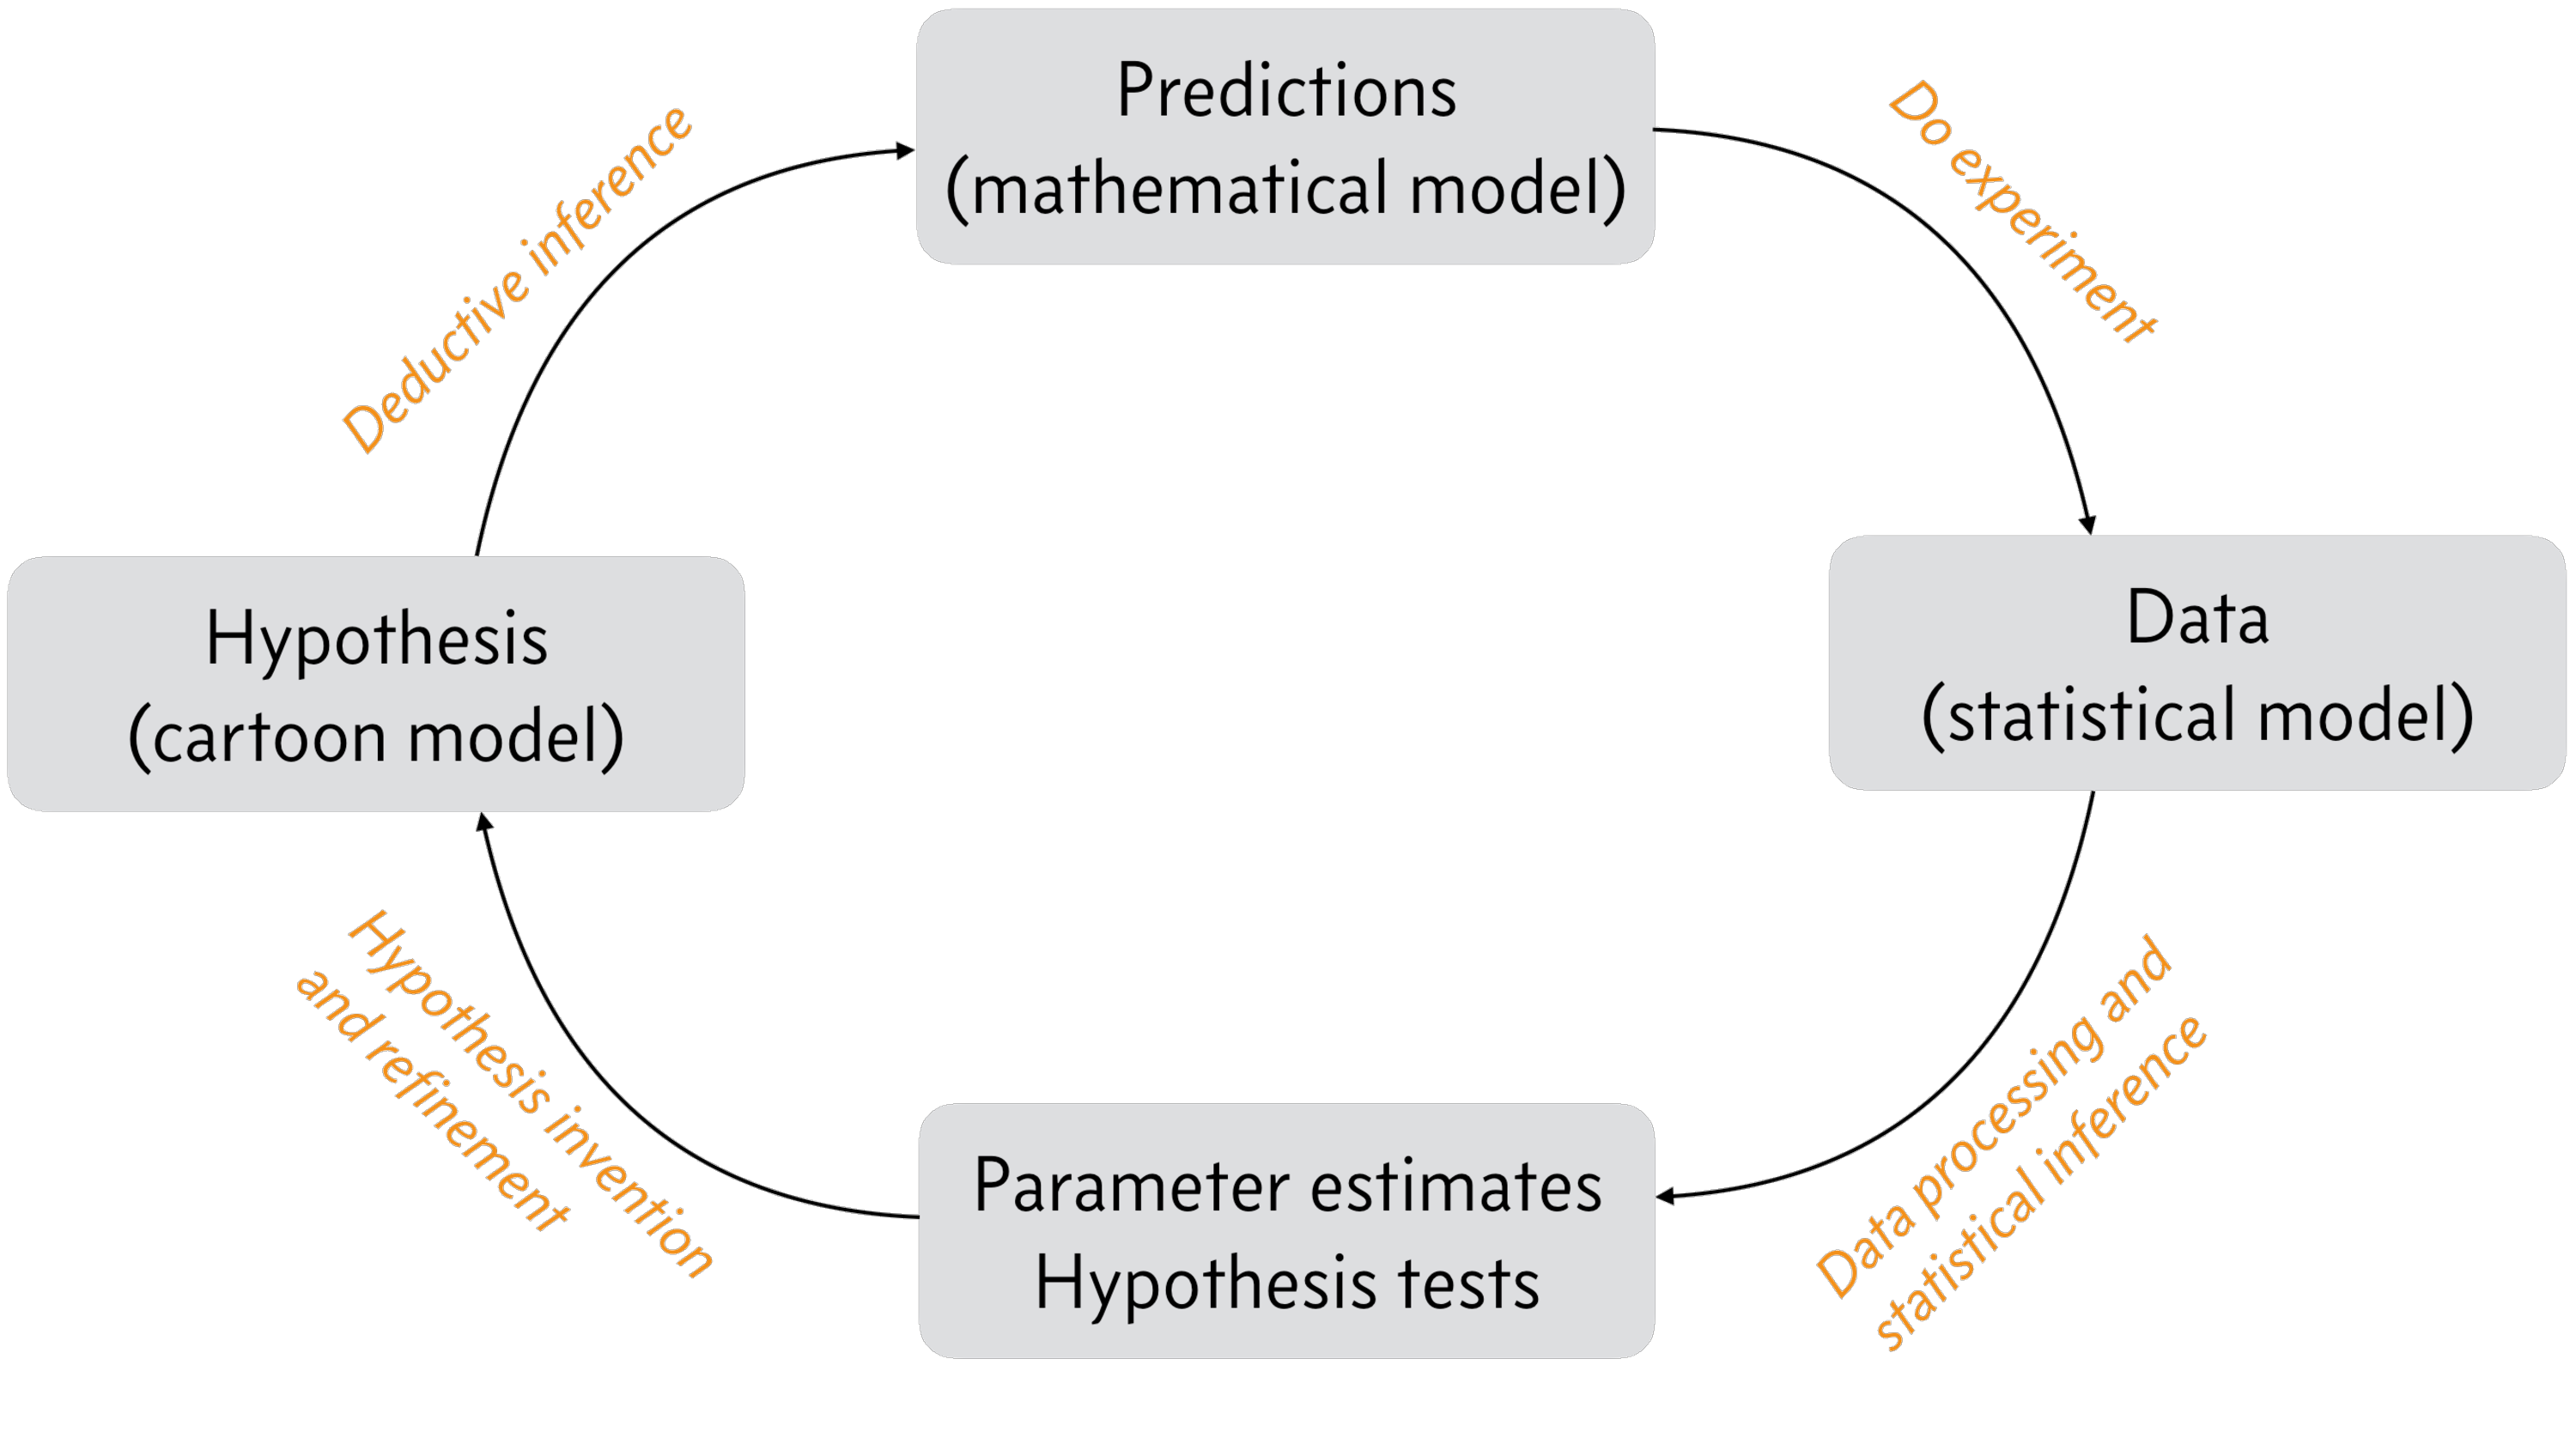
\includegraphics{images/cycle_of_science} 

}

\caption{Rappresentazione schematica del processo scientifico (figura adattata dalla Fig. 1.1 di P. Gregory, Bayesian Logical Data Analysis for the Physical Sciences, Cambridge, 2005).}\label{fig:cycle-of-science}
\end{figure}

Consideriamo i compiti e le fasi dell'indagine scientifica. Iniziamo in basso a sinistra.

\begin{itemize}
\item
  \emph{Invenzione e perfezionamento delle ipotesi.} In questa fase del processo scientifico, i ricercatori pensano ai fenomeni naturali, a ciò che è presente nella letteratura scientifica, ai risultati dei loro esperimenti, e formulano ipotesi o teorie che possono essere valutare mediante esperimenti empirici. Questo passaggio richiede innovazione e creatività.
\item
  L'\emph{inferenza deduttiva} procede in maniera deterministica dai fatti alle conclusioni. Ad esempio, se dico che tutti gli uomini sono mortali e che Socrate è un uomo, allora posso concludere deduttivamente che Socrate è mortale. Quando i ricercatori progettano gli esperimenti in base alle teorie, usano la logica deduttiva per dire: ``Se A è vero, allora B deve essere vero'', dove \(A\) è l'ipotesi teorica e \(B\) è l'osservazione sperimentale.
\item
  \emph{Esecuzione degli esperimenti.} Questa fase richiede molte risorse (tempo e denaro). Richiede anche innovazione e creatività. Nello specifico, i ricercatori devono pensare attentamente a come costruire l'esperimento necessario per verificare la teoria di interesse. Quale risultato dell'esperimento si ottengono i dati.
\item
  L'\emph{inferenza induttiva} procede dalle osservazioni ai fatti. Se pensiamo ai fatti come a ciò che governa o genera le osservazioni, allora l'induzione è una sorta di inferenza inversa. Supponiamo di avere osservato \(B\). Questo rende \(A\) vero? Non necessariamente. Ma può rendere \(A\) più plausibile. Questo è un sillogismo debole. Ad esempio, si consideri la seguente coppia ipotesi/osservazioni.

  \begin{itemize}
  \item
    \(A\) = L'iniezione di acque reflue dopo la fratturazione idraulica, nota come fracking, può portare a una maggiore frequenza di terremoti.
  \item
    \(B\) = La frequenza dei terremoti in Oklahoma è aumentata di 100 volte dal 2010, quando il fracking è diventato una pratica comune.
  \item
    Poiché \(B\) è stato osservato, \(A\) è più plausibile. \(A\) non è necessariamente vero, ma è più plausibile.
  \end{itemize}
\item
  L'\emph{inferenza statistica} è un tipo di inferenza induttiva che è specificamente formulata come un problema inverso. L'inferenza statistica è quell'insieme di procedure che hanno lo scopo di quantificare quanto più plausibile sia \(A\) dopo aver osservato \(B\). Per svolgere l'inferenza statistica è dunque necessario quantificare tale plausibilità. Lo strumento che ci consente di fare questo è la teoria delle probabilità.
\end{itemize}

L'inferenza statistica è l'aspetto del processo dell'indagine scientifica che costituisce il tema centrale di questo insegnamento. Il risultato dell'inferenza statistica è la conoscenza di quanto siano plausibili le ipotesi e le stime dei parametri sotto le ipotesi considerate. Ma l'inferenza statistica richiede una teoria delle probabilità, laddove la teoria delle probabilità può essere vista come una generalizzazione della logica. A causa di questa connessione con la logica, e del suo ruolo cruciale nella scienza, E. T. Jaynes ha dichiarato che ``la probabilità è la logica della scienza''. Per potere trattare i temi di base dell'inferenza statistica è dunque necessario esaminare preliminarmente alcune nozioni della teoria delle probabilità.

\hypertarget{che-cosuxe8-la-probabilituxe0}{%
\section{Che cos'è la probabilità?}\label{che-cosuxe8-la-probabilituxe0}}

La definizione della probabilità è un problema estremamente dibattuto ed aperto. Sono state fornite due possibili soluzioni al problema di definire il concetto di probabilità.

\begin{enumerate}
\def\labelenumi{(\alph{enumi})}
\item
  La natura della probabilità è ``ontologica'' (ovvero, basata sulla metafisica): la probabilità è una proprietà della della realtà, del mondo, di come sono le cose, indipendentemente dalla nostra esperienza. È una visione che qualcuno chiama ``oggettiva''.
\item
  La natura della probabilità è ``epistemica'' (ovvero, basata sulla conoscenza): la probabilità si riferisce alla conoscenza che abbiamo del mondo, non al mondo in sé. Di conseguenza è detta, in contrapposizione alla precedente definizione, ``soggettiva''.
\end{enumerate}

In termini epistemici, la probabilità fornisce una misura della nostra incertezza sul verificarsi di un fenomeno, alla luce delle informazioni disponibili. Potremmo dire che c'è una ``scala'' naturale che ha per estremi il vero (1: evento certo) da una parte ed il falso (0: evento impossibile) dall'altra. La probabilità è la quantificazione di questa scala: quantifica lo stato della nostra incertezza rispetto al contenuto di verità di una proposizione (ovvero, quantifica la plausibilità di una proposizione).

\begin{itemize}
\item
  Nell'interpretazione frequentista della probabilità, la probabilità \(P(A)\) rappresenta la frequenza relativa a lungo termine nel caso di un grande numero di ripetizioni di un esperimento casuale sotto le medesime condizioni. L'evento \(A\) deve essere una proposizione relativa alle variabili casuali\footnote{Viene stressata qui l'idea che ciò di cui parliamo è qualcosa che emerge nel momento in cui è possibile ripetere l'esperimento casuale tante volte sotto le medesime condizioni. Le variabili casuali, infatti, forniscono una quantificazione dei risultati che si ottengono ripetendo tante volte l'esperimento casuale sotto le medesime condizioni.}.
\item
  Nell'interpretazione bayesiana della probabilità \(P(A)\) rappresenta il grado di credenza, o plausibilità, a proposito di \(A\), dove \(A\) può essere qualsiasi proposizione logica.
\end{itemize}

In questo insegnamento utilizzeremo l'interpretazione bayesiana della probabilità. Possiamo citare De Finetti, ad esempio, il quale ha formulato la seguente definizione ``soggettiva'' di probabilità la quale risulta applicabile anche ad esperimenti casuali i cui eventi elementari non siano ritenuti ugualmente possibili e che non siano necessariamente ripetibili più volte sotto le stesse condizioni:

\begin{definition}
La probabilità di un evento \(E\) è la quota \(p(E)\) che un individuo reputa di dover pagare ad un banco per ricevere ``1'' ovvero ``0'' verificandosi o non verificandosi \(E\). Le valutazioni di probabilità degli eventi devono rispondere ai pricipi di equità e coerenza.
\end{definition}

I principi di equità e coerenza sono definiti come segue.

\begin{definition}
Una scommessa risponde ai pricipi di \emph{equità} se il ruolo di banco e giocatore sono scambiabili in ogni momento del gioco e sempre alle stesse condizioni; \emph{coerenza} se non vi sono combinazioni di scommesse che consentano (sia al banco che al giocatore) di realizzare perdite o vincite certe.
\end{definition}

Secondo \citet{definetti1931prob}, \emph{``nessuna scienza ci permetterà di dire: il tale fatto accadrà, andrà così e così, perché ciò è conseguenza di tale legge, e tale legge è una verità assoluta, ma tanto meno ci condurrà a concludere scetticamente: la verità assoluta non esiste, e quindi tale fatto può accadere e può non accadere, può andare così e può andare in tutt'altro modo, nulla io ne so. Quel che si potrà dire è questo: io prevedo che il tale fatto avverrà, e avverrà nel tal modo, perché l'esperienza del passato e l'elaborazione scientifica cui il pensiero dell'uomo l'ha sottoposta mi fanno sembrare ragionevole questa previsione.''}

In altri termini, de Finetti ritiene che la probabilità debba essere concepita non come una proprietà ``oggettiva'' dei fenomeni (``la probabilità di un fenomeno ha un valore determinato che dobbiamo solo scoprire''), ma bensì come il ``grado di fiducia -- in inglese \emph{degree of belief} -- di un dato soggetto, in un dato istante e con un dato insieme d'informazioni, riguardo al verificarsi di un evento''. Per denotare sia la probabilità (soggettiva) di un evento sia il concetto di \emph{valore atteso} (che descriveremo in seguito), \citet{definetti1970teoria} utilizza il termine ``previsione'' (e lo stesso simbolo \(P\)): \emph{``la previsione {[}\(\dots\){]} consiste nel considerare ponderatamente tutte le alternative possibili per ripartire fra di esse nel modo che parrà più appropriato le proprie aspettative, le proprie sensazioni di probabilità.''}

\hypertarget{variabili-casuali-e-probabilituxe0-di-un-evento}{%
\section{Variabili casuali e probabilità di un evento}\label{variabili-casuali-e-probabilituxe0-di-un-evento}}

Esaminiamo qui di seguito alcuni concetti di base della teoria delle probabilità.

\hypertarget{variabili-casuali}{%
\subsection{Variabili casuali}\label{variabili-casuali}}

Sia \(Y\) il risultato del lancio di moneta equilibrata, non di un generico lancio di una moneta, ma un'istanza specifica del lancio di una specifica moneta in un dato momento. Definita in questo modo, \(Y\) è una \emph{variabile casuale}, ovvero una variabile che assume valori diversi con probabilità diverse. Se la moneta è equilibrata, c'è una probabilità del 50\% che il lancio della moneta dia come risultato ``testa'' e una probabilità del 50\% che dia come risultato ``croce''.

Per facilitare la trattazione, le variabili casuali assumono solo valori numerici. Per lo specifico lancio della moneta in questione, diciamo, ad esempio, che la variabile casuale \(Y\) assume il valore 1 se esce testa e il valore 0 se esce croce.

\hypertarget{eventi-e-probabilituxe0}{%
\subsection{Eventi e probabilità}\label{eventi-e-probabilituxe0}}

Nella teoria delle probabilità il risultato ``testa'' nel lancio di una moneta è chiamato \emph{evento}.\footnote{Per un ripasso delle nozioni di base della teoria degli insiemi, si veda l'Appendice \ref{insiemistica}.} Ad esempio, \(Y\) = 1 denota l'evento in cui il lancio di una moneta produce come risultato testa.

Il funzionale \(Pr[·]\) definisce la probabilità di un evento. Ad esempio, per il lancio di una moneta equilibrata, la probabilità dell'evento ``il risultato del lancio della moneta è testa'' è scritta come

\[
Pr[Y = 1] = 0.5.
\] Se la moneta è equilibrata dobbiamo anche avere \(Pr[Y = 0] = 0.5\). I due eventi \emph{Y} = 1 e \(Y\) = 0 sono \emph{mutuamente esclusivi} nel senso che non possono entrambi verificarsi contemporaneamente. Nella notazione probabilistica,

\[
Pr[Y = 1\; e \; Y = 0] = 0.
\] Gli eventi \(Y\) = 1 e \(Y\) = 0 di dicono \emph{esaustivi}, nel senso che almeno uno di essi deve verificarsi e nessun altro tipo di evento è possibile. Nella notazione probabilistica,

\[
Pr[Y = 1\; o \; Y = 0] = 1.
\] Il connettivo logico ``e'' specifica eventi \emph{congiunti}, ovvero eventi che possono verificarsi contemporaneamente (eventi \emph{compatibili}) e per i quali, perciò, la probabilità della loro congiunzione è \(Pr(A \; e \; B) > 0\). Il connettivo logico ``o'' specifica eventi \emph{disgiunti}, ovvero eventi che non possono verificarsi contemporaneamente (eventi \emph{incompatibili}) e per i quali, perciò, la probabilità della loro congiunzione è \(P(A \; e \; B) = 0\).

\hypertarget{spazio-campionario-e-risultati-possibili}{%
\section{Spazio campionario e risultati possibili}\label{spazio-campionario-e-risultati-possibili}}

Anche se il lancio di una moneta produce sempre uno specifico risultato nel mondo reale, noi possiamo anche immaginare i possibili risultati alternativi che si sarebbero potuti osservare. Quindi, anche se in uno specifico lancio la moneta dà testa (\(Y\) = 1), possiamo immaginare la possibilità che il lancio possa avere prodotto croce (\(Y\) = 0). Tale ragionamento controfattuale è la chiave per comprendere la teoria delle probabilità e l'inferenza statistica.

I risultati possibili che si possono osservare come conseguenza del lancio di una moneta determinano i valori possibili che la variabile casuale può assumere. L'insieme di tutti i risultati possibili è chiamato \emph{spazio campionario}. Lo spazio campionario può essere concettualizzato come un'urna contenente una pallina per ogni possibile risultato del lancio della moneta. Su ogni pallina è scritto il valore della variabile casuale. Uno specifico lancio di una moneta -- ovvero, l'osservazione di uno specifico valore di una variabile casuale -- è chiamato \emph{esperimento casuale}.

Il lancio di un dado ci fornisce l'esempio di un altro esperimento casuale. Supponiamo di essere interessati all'evento ``il lancio del dado produce un numero dispari''. Un \emph{evento} seleziona un sottoinsieme dello spazio campionario: in questo caso, l'insieme dei risultati \(\{1, 3, 5\}\). Se esce 3, per esempio, diciamo che si è verificato l'evento ``dispari'' (ma l'evento ``dispari'' si sarebbe anche verificato anche se fosse uscito 1 o 5).

\hypertarget{usare-la-simulazione-per-stimare-le-probabilituxe0}{%
\section{Usare la simulazione per stimare le probabilità}\label{usare-la-simulazione-per-stimare-le-probabilituxe0}}

I metodi basati sulla simulazione ci consentono di stimare le probabilità degli eventi in un modo diretto se siamo in grado di generare realizzazioni molteplici e casuali delle variabili casuali coinvolte nelle definizioni degli eventi. Per simulare il lancio di una moneta equilibrata in R iniziamo a definire un vettore che contiene i possibili risultati del lancio della moneta (ovvero i possibili valori della variabile casuale \(Y\)):

\begin{Shaded}
\begin{Highlighting}[]
\NormalTok{coin }\OtherTok{\textless{}{-}} \FunctionTok{c}\NormalTok{(}\DecValTok{0}\NormalTok{, }\DecValTok{1}\NormalTok{)}
\end{Highlighting}
\end{Shaded}

\noindent L'estrazione casuale di uno di questi due possibili valori (ovvero, la simulazione di uno specifico lancio di una moneta) si realizza con la funzione \texttt{sample()}:

\begin{Shaded}
\begin{Highlighting}[]
\FunctionTok{sample}\NormalTok{(coin, }\AttributeTok{size =} \DecValTok{1}\NormalTok{)}
\CommentTok{\#\textgreater{} [1] 0}
\end{Highlighting}
\end{Shaded}

\noindent In maniera equivalente, lo stesso risultato si ottiene mediante l'istruzione

\begin{Shaded}
\begin{Highlighting}[]
\FunctionTok{rbinom}\NormalTok{(}\DecValTok{1}\NormalTok{, }\DecValTok{1}\NormalTok{, }\FloatTok{0.5}\NormalTok{)}
\CommentTok{\#\textgreater{} [1] 1}
\end{Highlighting}
\end{Shaded}

Supponiamo di ripetere questo esperimento casuale 100 volte e di registrare i risultati così ottenuti. La stima della probabilità dell'evento \(Pr[Y = 1]\) è data dalla frequenza relativa del numero di volte in cui abbiamo osservato l'evento di interesse (\(Y = 1\)):

\begin{Shaded}
\begin{Highlighting}[]
\NormalTok{M }\OtherTok{\textless{}{-}} \DecValTok{10}
\NormalTok{y }\OtherTok{\textless{}{-}} \FunctionTok{rep}\NormalTok{(}\ConstantTok{NA}\NormalTok{, M)}
\ControlFlowTok{for}\NormalTok{ (m }\ControlFlowTok{in} \DecValTok{1}\SpecialCharTok{:}\NormalTok{M) \{}
\NormalTok{  y[m] }\OtherTok{=} \FunctionTok{rbinom}\NormalTok{(}\DecValTok{1}\NormalTok{, }\DecValTok{1}\NormalTok{, }\FloatTok{0.5}\NormalTok{)}
\NormalTok{\}}
\NormalTok{estimate }\OtherTok{=} \FunctionTok{sum}\NormalTok{(y) }\SpecialCharTok{/}\NormalTok{ M}

\FunctionTok{cat}\NormalTok{(}\StringTok{"estimated Pr[Y = 1] ="}\NormalTok{, estimate)}
\CommentTok{\#\textgreater{} estimated Pr[Y = 1] = 0.5}
\end{Highlighting}
\end{Shaded}

\noindent Ripetiamo questa procedura 10 volte.

\begin{Shaded}
\begin{Highlighting}[]
\NormalTok{flip\_coin }\OtherTok{\textless{}{-}} \ControlFlowTok{function}\NormalTok{(M) \{}
\NormalTok{  y }\OtherTok{\textless{}{-}} \FunctionTok{rep}\NormalTok{(}\ConstantTok{NA}\NormalTok{, M)}
  \ControlFlowTok{for}\NormalTok{ (m }\ControlFlowTok{in} \DecValTok{1}\SpecialCharTok{:}\NormalTok{M) \{}
\NormalTok{    y[m] }\OtherTok{=} \FunctionTok{rbinom}\NormalTok{(}\DecValTok{1}\NormalTok{, }\DecValTok{1}\NormalTok{, }\FloatTok{0.5}\NormalTok{)}
\NormalTok{  \}}
\NormalTok{  estimate }\OtherTok{\textless{}{-}} \FunctionTok{sum}\NormalTok{(y) }\SpecialCharTok{/}\NormalTok{ M}
  \FunctionTok{cat}\NormalTok{(}\StringTok{"estimated Pr[Y = 1] ="}\NormalTok{, estimate, }\StringTok{"}\SpecialCharTok{\textbackslash{}n}\StringTok{"}\NormalTok{)}
\NormalTok{\}}
\end{Highlighting}
\end{Shaded}

\begin{Shaded}
\begin{Highlighting}[]
\ControlFlowTok{for}\NormalTok{(i }\ControlFlowTok{in} \DecValTok{1}\SpecialCharTok{:}\DecValTok{10}\NormalTok{) \{}
  \FunctionTok{flip\_coin}\NormalTok{(}\DecValTok{10}\NormalTok{)}
\NormalTok{\}}
\CommentTok{\#\textgreater{} estimated Pr[Y = 1] = 0.5 }
\CommentTok{\#\textgreater{} estimated Pr[Y = 1] = 0.3 }
\CommentTok{\#\textgreater{} estimated Pr[Y = 1] = 0.7 }
\CommentTok{\#\textgreater{} estimated Pr[Y = 1] = 0.5 }
\CommentTok{\#\textgreater{} estimated Pr[Y = 1] = 0.5 }
\CommentTok{\#\textgreater{} estimated Pr[Y = 1] = 0.6 }
\CommentTok{\#\textgreater{} estimated Pr[Y = 1] = 0.5 }
\CommentTok{\#\textgreater{} estimated Pr[Y = 1] = 0.8 }
\CommentTok{\#\textgreater{} estimated Pr[Y = 1] = 0.4 }
\CommentTok{\#\textgreater{} estimated Pr[Y = 1] = 0.5}
\end{Highlighting}
\end{Shaded}

\noindent Dato che la moneta è equilibrata, la stima delle probabilità dell'evento \(Pr[Y = 1]\) è simile a al valore che ci aspettiamo (\(Pr[Y = 1]\) = 0.5), ma il risultato ottenuto nelle varie simulazioni non è sempre esatto. Proviamo ad aumentare il numero di lanci in ciascuna simulazione:

\begin{Shaded}
\begin{Highlighting}[]
\ControlFlowTok{for}\NormalTok{(i }\ControlFlowTok{in} \DecValTok{1}\SpecialCharTok{:}\DecValTok{10}\NormalTok{) \{}
  \FunctionTok{flip\_coin}\NormalTok{(}\DecValTok{100}\NormalTok{)}
\NormalTok{\}}
\CommentTok{\#\textgreater{} estimated Pr[Y = 1] = 0.44 }
\CommentTok{\#\textgreater{} estimated Pr[Y = 1] = 0.53 }
\CommentTok{\#\textgreater{} estimated Pr[Y = 1] = 0.43 }
\CommentTok{\#\textgreater{} estimated Pr[Y = 1] = 0.58 }
\CommentTok{\#\textgreater{} estimated Pr[Y = 1] = 0.5 }
\CommentTok{\#\textgreater{} estimated Pr[Y = 1] = 0.41 }
\CommentTok{\#\textgreater{} estimated Pr[Y = 1] = 0.51 }
\CommentTok{\#\textgreater{} estimated Pr[Y = 1] = 0.49 }
\CommentTok{\#\textgreater{} estimated Pr[Y = 1] = 0.5 }
\CommentTok{\#\textgreater{} estimated Pr[Y = 1] = 0.57}
\end{Highlighting}
\end{Shaded}

\noindent In questo secondo caso, gli errori tendono ad essere più piccoli della simulazione precedente. Cosa succede se in ciascuna simulazione esaminiamo i risultati di 10,000 lanci della moneta?

\begin{Shaded}
\begin{Highlighting}[]
\ControlFlowTok{for}\NormalTok{(i }\ControlFlowTok{in} \DecValTok{1}\SpecialCharTok{:}\DecValTok{10}\NormalTok{) \{}
  \FunctionTok{flip\_coin}\NormalTok{(}\FloatTok{1e4}\NormalTok{)}
\NormalTok{\}}
\CommentTok{\#\textgreater{} estimated Pr[Y = 1] = 0.5029 }
\CommentTok{\#\textgreater{} estimated Pr[Y = 1] = 0.4886 }
\CommentTok{\#\textgreater{} estimated Pr[Y = 1] = 0.4956 }
\CommentTok{\#\textgreater{} estimated Pr[Y = 1] = 0.49 }
\CommentTok{\#\textgreater{} estimated Pr[Y = 1] = 0.5032 }
\CommentTok{\#\textgreater{} estimated Pr[Y = 1] = 0.5051 }
\CommentTok{\#\textgreater{} estimated Pr[Y = 1] = 0.4928 }
\CommentTok{\#\textgreater{} estimated Pr[Y = 1] = 0.4968 }
\CommentTok{\#\textgreater{} estimated Pr[Y = 1] = 0.4991 }
\CommentTok{\#\textgreater{} estimated Pr[Y = 1] = 0.4976}
\end{Highlighting}
\end{Shaded}

\noindent Ora le stime ottenute sono molto vicine alla vera probabilità che vogliamo stimare (cioè 0.5, perché la moneta è equilibrata). I risultati delle simulazioni precedenti pongono dunque il problema di determinare quale sia il numero di lanci di cui abbiamo bisogno per assicurarci che le stime siano accurate (ovvero, vicine al valore corretto della probabilità)

\hypertarget{la-legge-dei-grandi-numeri}{%
\section{La legge dei grandi numeri}\label{la-legge-dei-grandi-numeri}}

La visualizzazione mediante grafici contribuisce alla comprensione dei concetti della statistica e della teoria delle probabilità. Un modo per descrivere ciò che accade all'aumentare del numero \(M\) di ripetizioni del lancio della moneta consiste nel registrare la stima della probabilità dell'evento \(Pr[Y = 1]\) in funzione del numero di ripetizioni dell'esperimento casuale per ogni \(m \in 1 : M.\) Un grafico dell'andamento della stima di \(Pr[Y = 1]\) in funzione di \(m\) si ottiene nel modo seguente.

\begin{Shaded}
\begin{Highlighting}[]
\NormalTok{nrep }\OtherTok{\textless{}{-}} \FloatTok{1e4}
\NormalTok{estimate }\OtherTok{\textless{}{-}} \FunctionTok{rep}\NormalTok{(}\ConstantTok{NA}\NormalTok{, nrep)}
\NormalTok{flip\_coin }\OtherTok{\textless{}{-}} \ControlFlowTok{function}\NormalTok{(m) \{}
\NormalTok{  y }\OtherTok{\textless{}{-}} \FunctionTok{rbinom}\NormalTok{(m, }\DecValTok{1}\NormalTok{, }\FloatTok{0.5}\NormalTok{)}
\NormalTok{  phat }\OtherTok{\textless{}{-}} \FunctionTok{sum}\NormalTok{(y) }\SpecialCharTok{/}\NormalTok{ m}
\NormalTok{  phat}
\NormalTok{\}}
\ControlFlowTok{for}\NormalTok{(i }\ControlFlowTok{in} \DecValTok{1}\SpecialCharTok{:}\NormalTok{nrep) \{}
\NormalTok{  estimate[i] }\OtherTok{\textless{}{-}} \FunctionTok{flip\_coin}\NormalTok{(i)}
\NormalTok{\}}
\NormalTok{d }\OtherTok{\textless{}{-}} \FunctionTok{data.frame}\NormalTok{(}
  \AttributeTok{n =} \DecValTok{1}\SpecialCharTok{:}\NormalTok{nrep, }
\NormalTok{  estimate}
\NormalTok{)}
\NormalTok{d }\SpecialCharTok{\%\textgreater{}\%} 
  \FunctionTok{ggplot}\NormalTok{(}
    \FunctionTok{aes}\NormalTok{(}\AttributeTok{x =}\NormalTok{ n, }\AttributeTok{y =}\NormalTok{ estimate)}
\NormalTok{  ) }\SpecialCharTok{+}
  \FunctionTok{geom\_line}\NormalTok{() }\SpecialCharTok{+}
  \FunctionTok{theme}\NormalTok{(}\AttributeTok{legend.title =} \FunctionTok{element\_blank}\NormalTok{()) }\SpecialCharTok{+}
  \FunctionTok{labs}\NormalTok{(}
    \AttributeTok{x =} \StringTok{"Numero di lanci della moneta"}\NormalTok{, }
    \AttributeTok{y =} \StringTok{"Stima Pr[Y = 1]"}
\NormalTok{)}
\end{Highlighting}
\end{Shaded}

\begin{figure}[h]

{\centering 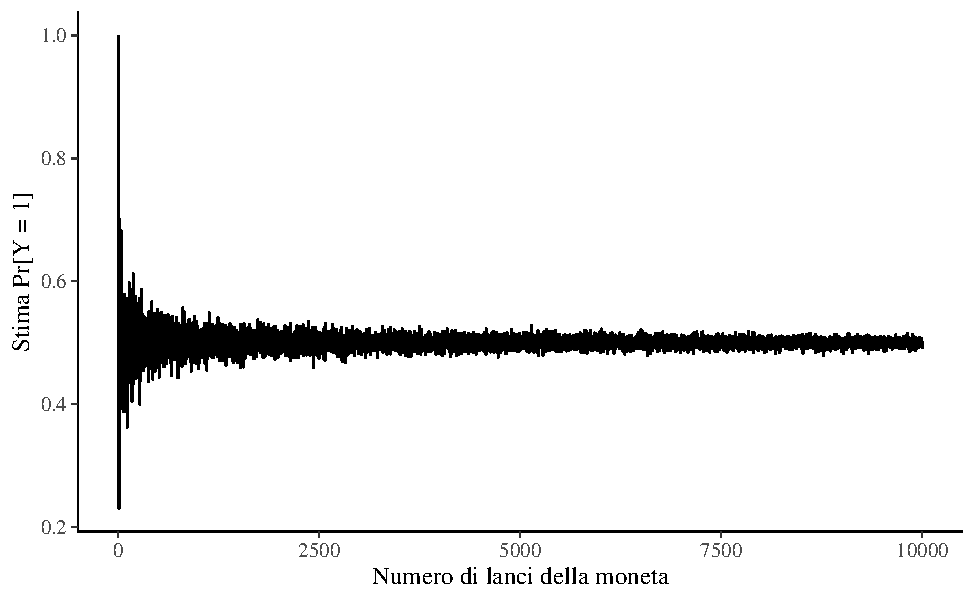
\includegraphics{ds4psy_files/figure-latex/legge-grandi-n-1-1} 

}

\caption{Stima della probabilità di successo in funzione del numero di lanci di una moneta.}\label{fig:legge-grandi-n-1}
\end{figure}

Dato che il grafico \ref{fig:legge-grandi-n-1} su una scala lineare non rivela chiaramente l'andamento della simulazione, utilizzeremo invece un grafico in cui sull'asse \(x\) è stata imposta una scala logaritmica. Con l'asse \(x\) su scala logaritmica, i valori tra 1 e 10 vengono tracciati all'incirca con la stessa ampiezza come nel caso dei valori tra 50 e 700, eccetera.

\begin{Shaded}
\begin{Highlighting}[]
\NormalTok{d }\SpecialCharTok{\%\textgreater{}\%} 
  \FunctionTok{ggplot}\NormalTok{(}
    \FunctionTok{aes}\NormalTok{(}\AttributeTok{x =}\NormalTok{ n, }\AttributeTok{y =}\NormalTok{ estimate)}
\NormalTok{  ) }\SpecialCharTok{+}
  \FunctionTok{geom\_line}\NormalTok{() }\SpecialCharTok{+}
  \FunctionTok{scale\_x\_log10}\NormalTok{(}
    \AttributeTok{breaks =} \FunctionTok{c}\NormalTok{(}\DecValTok{1}\NormalTok{, }\DecValTok{3}\NormalTok{, }\DecValTok{10}\NormalTok{, }\DecValTok{50}\NormalTok{, }\DecValTok{200}\NormalTok{, }
               \DecValTok{700}\NormalTok{, }\DecValTok{2500}\NormalTok{, }\DecValTok{10000}\NormalTok{)}
\NormalTok{  ) }\SpecialCharTok{+}
  \FunctionTok{theme}\NormalTok{(}\AttributeTok{legend.title =} \FunctionTok{element\_blank}\NormalTok{()) }\SpecialCharTok{+}
  \FunctionTok{labs}\NormalTok{(}
    \AttributeTok{x =} \StringTok{"Numero di lanci della moneta"}\NormalTok{, }
    \AttributeTok{y =} \StringTok{"Stima Pr[Y = 1]"}
\NormalTok{)}
\end{Highlighting}
\end{Shaded}

\begin{figure}[h]

{\centering 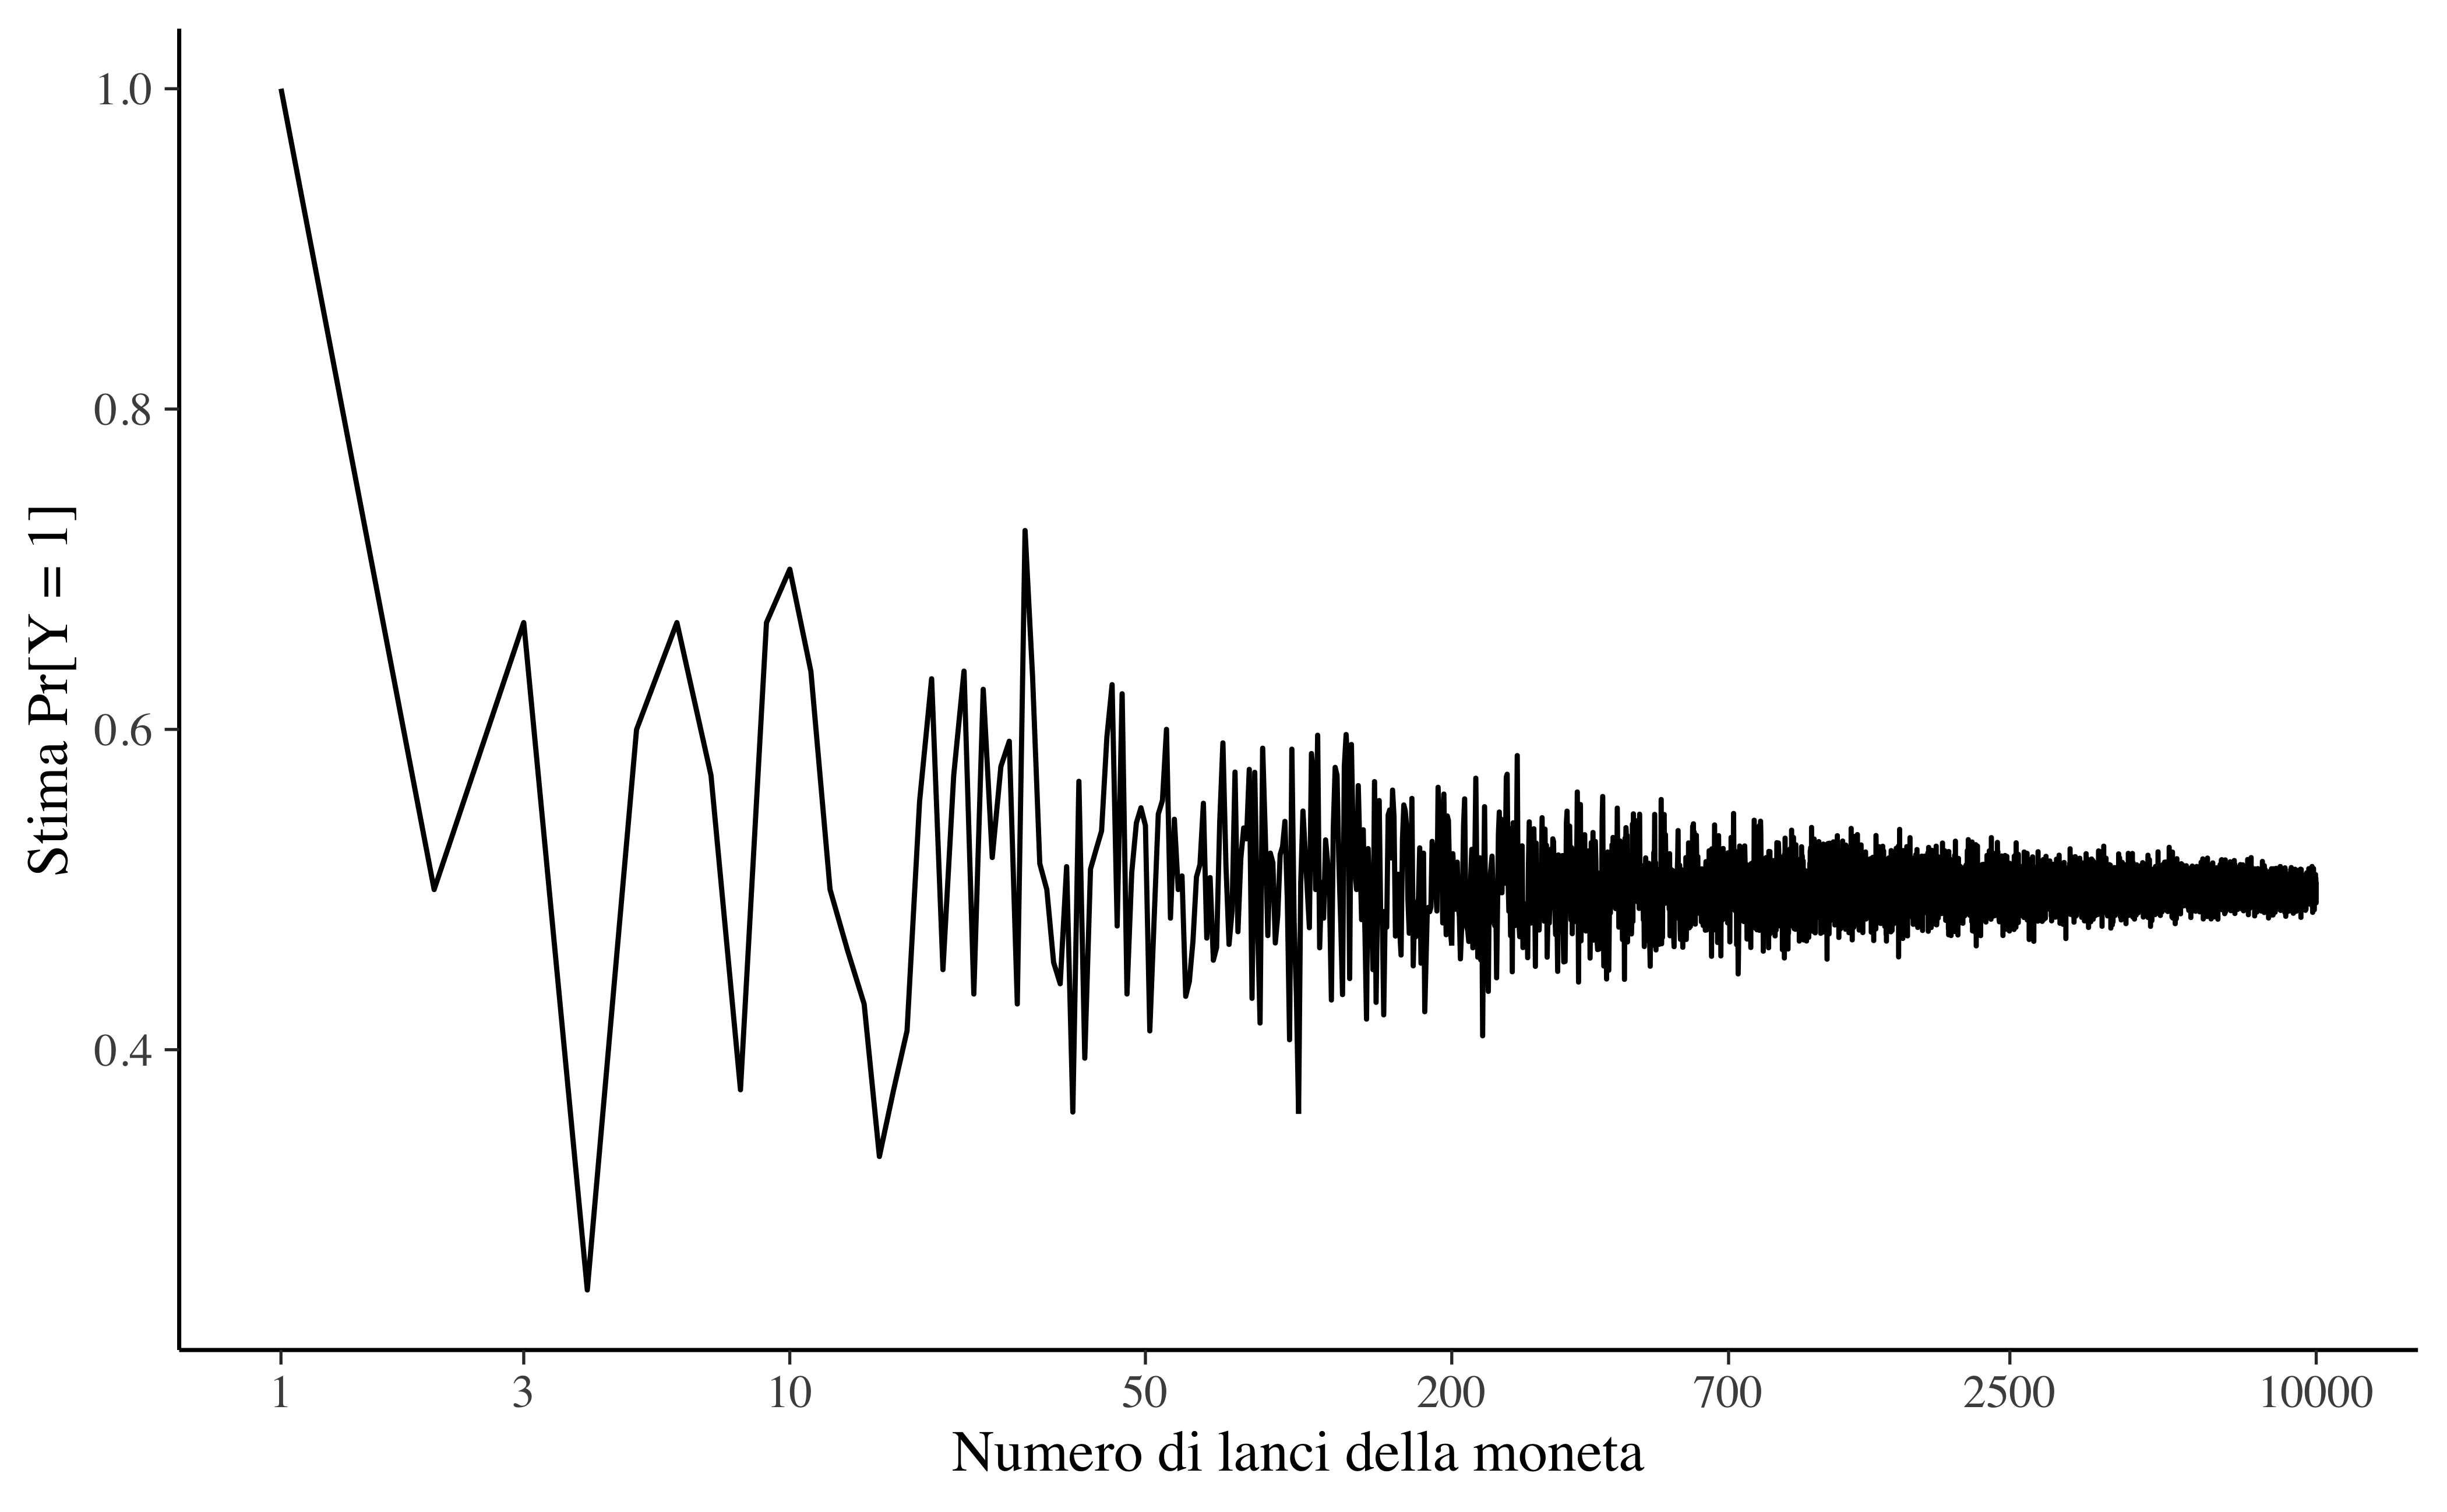
\includegraphics{ds4psy_files/figure-latex/legge-grandi-n-2-1} 

}

\caption{Stima della probabilità di successo in funzione del numero di lanci di una moneta -- scala logaritmica.}\label{fig:legge-grandi-n-2}
\end{figure}

La \emph{legge dei grandi numeri} ci dice che all'aumentare del numero di ripetizioni dell'esperimento casuale la media dei risultati ottenuti tenderà ad avvicinarsi al valore atteso man mano che verranno eseguite più prove. Nel caso presente, la figura \ref{fig:legge-grandi-n-2} mostra appunto che, all'aumentare del numero \emph{M} di lanci della moneta, la stima di \(Pr[Y = 1]\) tende a convergere al vero valore di 0.5.

\hypertarget{variabili-casuali-multiple}{%
\section{Variabili casuali multiple}\label{variabili-casuali-multiple}}

Le variabili casuali non esistono isolatamente. Abbiamo iniziato con una singola variabile casuale \emph{Y} che rappresenta il risultato di un singolo, specifico lancio di una moneta equlibrata. Ma supponiamo ora di lanciare la moneta tre volte. Ciò suggerisce che possiamo avere le variabili casuali \(Y_1 , Y_2 , Y_3\) che rappresentano i risultati di ciascuno dei lanci. Possiamo assumere che ogni lancio sia indipendente, ovvero che non dipenda dal risultato degli altri lanci. Ognuna di queste variabili \(Y_n\) per \(n \in 1:3\) ha \(Pr[Y_n =1]=0.5\) e \(Pr[Y_n =0]=0.5\). Possiamo combinare più variabili casuali usando le operazioni aritmetiche. Se \(Y_1 , Y_2, Y_3\) sono variabili casuali che rappresentano tre lanci di una moneta equilibrata (o un lancio di tre monete equilibrate), possiamo definire la somma di tali variabili casuali come

\[
Z = Y_1 + Y_2 + Y_3.
\] \noindent Possiamo simulare i valori assunti dalla variabile casuale \emph{Z} simulando i valori di \(Y_1, Y_2, Y_3\) per poi sommarli.

\begin{Shaded}
\begin{Highlighting}[]
\NormalTok{y1 }\OtherTok{\textless{}{-}} \FunctionTok{rbinom}\NormalTok{(}\DecValTok{1}\NormalTok{, }\DecValTok{1}\NormalTok{, }\FloatTok{0.5}\NormalTok{)}
\NormalTok{y2 }\OtherTok{\textless{}{-}} \FunctionTok{rbinom}\NormalTok{(}\DecValTok{1}\NormalTok{, }\DecValTok{1}\NormalTok{, }\FloatTok{0.5}\NormalTok{)}
\NormalTok{y3 }\OtherTok{\textless{}{-}} \FunctionTok{rbinom}\NormalTok{(}\DecValTok{1}\NormalTok{, }\DecValTok{1}\NormalTok{, }\FloatTok{0.5}\NormalTok{)}
\FunctionTok{c}\NormalTok{(y1, y2, y3)}
\CommentTok{\#\textgreater{} [1] 0 0 1}
\NormalTok{z }\OtherTok{\textless{}{-}} \FunctionTok{sum}\NormalTok{(}\FunctionTok{c}\NormalTok{(y1, y2, y3))}
\FunctionTok{cat}\NormalTok{(}\StringTok{"z ="}\NormalTok{, z, }\StringTok{"}\SpecialCharTok{\textbackslash{}n}\StringTok{"}\NormalTok{)}
\CommentTok{\#\textgreater{} z = 1}
\end{Highlighting}
\end{Shaded}

\noindent ovvero,

\begin{Shaded}
\begin{Highlighting}[]
\NormalTok{y }\OtherTok{\textless{}{-}} \FunctionTok{rep}\NormalTok{(}\ConstantTok{NA}\NormalTok{, }\DecValTok{3}\NormalTok{)}
\ControlFlowTok{for}\NormalTok{ (i }\ControlFlowTok{in} \DecValTok{1}\SpecialCharTok{:}\DecValTok{3}\NormalTok{) \{}
\NormalTok{  y[i] }\OtherTok{\textless{}{-}} \FunctionTok{rbinom}\NormalTok{(}\DecValTok{1}\NormalTok{, }\DecValTok{1}\NormalTok{, }\FloatTok{0.5}\NormalTok{)}
\NormalTok{\}}
\NormalTok{y}
\CommentTok{\#\textgreater{} [1] 1 0 0}
\NormalTok{z }\OtherTok{\textless{}{-}} \FunctionTok{sum}\NormalTok{(y)}
\FunctionTok{cat}\NormalTok{(}\StringTok{"z ="}\NormalTok{, z, }\StringTok{"}\SpecialCharTok{\textbackslash{}n}\StringTok{"}\NormalTok{)}
\CommentTok{\#\textgreater{} z = 1}
\end{Highlighting}
\end{Shaded}

\noindent oppure, ancora più semplicemente:

\begin{Shaded}
\begin{Highlighting}[]
\NormalTok{y }\OtherTok{\textless{}{-}} \FunctionTok{rbinom}\NormalTok{(}\DecValTok{3}\NormalTok{, }\DecValTok{1}\NormalTok{, }\FloatTok{0.5}\NormalTok{)}
\NormalTok{y}
\CommentTok{\#\textgreater{} [1] 0 1 1}
\NormalTok{z }\OtherTok{\textless{}{-}} \FunctionTok{sum}\NormalTok{(y)}
\FunctionTok{cat}\NormalTok{(}\StringTok{"z ="}\NormalTok{, z, }\StringTok{"}\SpecialCharTok{\textbackslash{}n}\StringTok{"}\NormalTok{)}
\CommentTok{\#\textgreater{} z = 2}
\end{Highlighting}
\end{Shaded}

\noindent Possiamo ripetere questa simulazione \(M = 1e5\) volte:

\begin{Shaded}
\begin{Highlighting}[]
\NormalTok{M }\OtherTok{\textless{}{-}} \FloatTok{1e5}
\NormalTok{z }\OtherTok{\textless{}{-}} \FunctionTok{rep}\NormalTok{(}\ConstantTok{NA}\NormalTok{, M)}
\ControlFlowTok{for}\NormalTok{(i }\ControlFlowTok{in} \DecValTok{1}\SpecialCharTok{:}\NormalTok{M) \{}
\NormalTok{  y }\OtherTok{\textless{}{-}} \FunctionTok{rbinom}\NormalTok{(}\DecValTok{3}\NormalTok{, }\DecValTok{1}\NormalTok{, }\FloatTok{0.5}\NormalTok{)}
\NormalTok{  z[i] }\OtherTok{\textless{}{-}} \FunctionTok{sum}\NormalTok{(y)}
\NormalTok{\}}
\end{Highlighting}
\end{Shaded}

\noindent e calcolare una stima della probabilità che la variabile casuale \(Z\) assuma i valori 0, 1, 2, 3:

\begin{Shaded}
\begin{Highlighting}[]
\FunctionTok{table}\NormalTok{(z) }\SpecialCharTok{/}\NormalTok{ M}
\CommentTok{\#\textgreater{} z}
\CommentTok{\#\textgreater{}      0      1      2      3 }
\CommentTok{\#\textgreater{} 0.1256 0.3750 0.3749 0.1245}
\end{Highlighting}
\end{Shaded}

Nel caso di 4 monete equilibrate, avremo:

\begin{Shaded}
\begin{Highlighting}[]
\NormalTok{M }\OtherTok{\textless{}{-}} \FloatTok{1e5}
\NormalTok{z }\OtherTok{\textless{}{-}} \FunctionTok{rep}\NormalTok{(}\ConstantTok{NA}\NormalTok{, M)}
\ControlFlowTok{for}\NormalTok{(i }\ControlFlowTok{in} \DecValTok{1}\SpecialCharTok{:}\NormalTok{M) \{}
\NormalTok{  y }\OtherTok{\textless{}{-}} \FunctionTok{rbinom}\NormalTok{(}\DecValTok{4}\NormalTok{, }\DecValTok{1}\NormalTok{, }\FloatTok{0.5}\NormalTok{)}
\NormalTok{  z[i] }\OtherTok{\textless{}{-}} \FunctionTok{sum}\NormalTok{(y)}
\NormalTok{\}}
\FunctionTok{table}\NormalTok{(z) }\SpecialCharTok{/}\NormalTok{ M}
\CommentTok{\#\textgreater{} z}
\CommentTok{\#\textgreater{}       0       1       2       3       4 }
\CommentTok{\#\textgreater{} 0.06213 0.25019 0.37400 0.25097 0.06271}
\end{Highlighting}
\end{Shaded}

Viene detta \emph{variabile casuale discreta} una variabile casuale le cui modalità possono essere costituite solo da numeri interi:

\[
\mathbb{Z} = \dots, -2, -1, 0, 1, 2, \dots
\]

\hypertarget{sec:fun-mass-prob}{%
\section{Funzione di massa di probabilità}\label{sec:fun-mass-prob}}

È conveniente avere una funzione che associa ogni possibile valore di una variabile casuale alla sua probabilità. In generale, ciò è possibile se e solo se la variabile casuale è discreta, così com'è stata definita nel Paragrafo precedente.

Ad esempio, se consideriamo \(Z = Y_1 + \dots + Y_4\) come il numero di risultati ``testa'' in 4 lanci della moneta, allora possiamo definire la seguente funzione:

\[
\begin{array}{rclll}
p_Z(0) & = & 1/16 & & \mathrm{TTTT}
\\
p_Z(1) & = & 4/16 & & \mathrm{HTTT, THTT, TTHT, TTTH}
\\
p_Z(2) & = & 6/16 & & \mathrm{HHTT, HTHT, HTTH, THHT, THTH, TTTH}
\\
p_Z(3) & = & 4/16 & & \mathrm{HHHT, HHTH, HTHH, THHH}
\\
p_Z(4) & = & 1/16 & & \mathrm{HHHH}
\end{array}
\]

Il lancio di quattro monete può produrre sedici possibili risultati. Dato che i lanci sono indipendenti e le monete sono equilibrate, ogni possibile risultato è ugualmente probabile. Nella tabella in alto, le sequenze dei risultati possibili del lancio delle 4 monete sono riportate nella colonna più a destra. Le probabilità si ottengono dividendo il numero di sequenze che producono lo stesso numero di eventi testa per il numero dei risultati possibili.

La funzione \(p_Z\) è stata costruita per mappare un valore \(u\) per \(Z\) alla probabilità dell'evento \(Z = u\). Convenzionalmente, queste probabilità sono scritte come

\[
p_Z(z) = \mbox{Pr}[Z = z].
\]

La parte a destra dell'uguale si può leggere come: ``la probabilità che la variabile casuale \(Z\) assuma il valore \(z\)''.

Una funzione definita come sopra è detta \emph{funzione di massa di probabilità} della variabile casuale \(Z\). Ad ogni variabile casuale discreta è associata un'unica funzione di massa di probabilità.

Una rappresentazione grafica della stima della funzione di massa di probabilità per l'esperimento casuale del lancio di quattro monete equilibrate è fornita nella figura \ref{fig:barplot-mdf-4coins}.

\begin{Shaded}
\begin{Highlighting}[]
\FunctionTok{set.seed}\NormalTok{(}\DecValTok{1234}\NormalTok{)}
\NormalTok{M }\OtherTok{\textless{}{-}} \FloatTok{1e5}
\NormalTok{nflips }\OtherTok{\textless{}{-}} \DecValTok{4}
\NormalTok{u }\OtherTok{\textless{}{-}} \FunctionTok{rbinom}\NormalTok{(M, nflips, }\FloatTok{0.5}\NormalTok{)}
\NormalTok{x }\OtherTok{\textless{}{-}} \DecValTok{0}\SpecialCharTok{:}\NormalTok{nflips}
\NormalTok{y }\OtherTok{\textless{}{-}} \FunctionTok{rep}\NormalTok{(}\ConstantTok{NA}\NormalTok{, nflips}\SpecialCharTok{+}\DecValTok{1}\NormalTok{)}
\ControlFlowTok{for}\NormalTok{ (n }\ControlFlowTok{in} \DecValTok{0}\SpecialCharTok{:}\NormalTok{nflips)}
\NormalTok{  y[n }\SpecialCharTok{+} \DecValTok{1}\NormalTok{] }\OtherTok{\textless{}{-}} \FunctionTok{sum}\NormalTok{(u }\SpecialCharTok{==}\NormalTok{ n) }\SpecialCharTok{/}\NormalTok{ M}
\NormalTok{bar\_plot }\OtherTok{\textless{}{-}}
  \FunctionTok{data.frame}\NormalTok{(}\AttributeTok{Z =}\NormalTok{ x, }\AttributeTok{count =}\NormalTok{ y) }\SpecialCharTok{\%\textgreater{}\%} 
  \FunctionTok{ggplot}\NormalTok{(}
    \FunctionTok{aes}\NormalTok{(}\AttributeTok{x =}\NormalTok{ Z, }\AttributeTok{y =}\NormalTok{ count)}
\NormalTok{  ) }\SpecialCharTok{+}
  \FunctionTok{geom\_bar}\NormalTok{(}\AttributeTok{stat =} \StringTok{"identity"}\NormalTok{) }\SpecialCharTok{+}
  \FunctionTok{scale\_x\_continuous}\NormalTok{(}
    \AttributeTok{breaks =} \DecValTok{0}\SpecialCharTok{:}\DecValTok{4}\NormalTok{,}
    \AttributeTok{labels =} \FunctionTok{c}\NormalTok{(}\DecValTok{0}\NormalTok{, }\DecValTok{1}\NormalTok{, }\DecValTok{2}\NormalTok{, }\DecValTok{3}\NormalTok{, }\DecValTok{4}\NormalTok{)}
\NormalTok{  ) }\SpecialCharTok{+}
  \FunctionTok{labs}\NormalTok{(}
    \AttributeTok{y =} \StringTok{"Probabilità stimata Pr[Z = z]"}
\NormalTok{)}
\NormalTok{bar\_plot}
\end{Highlighting}
\end{Shaded}

\begin{figure}[h]

{\centering 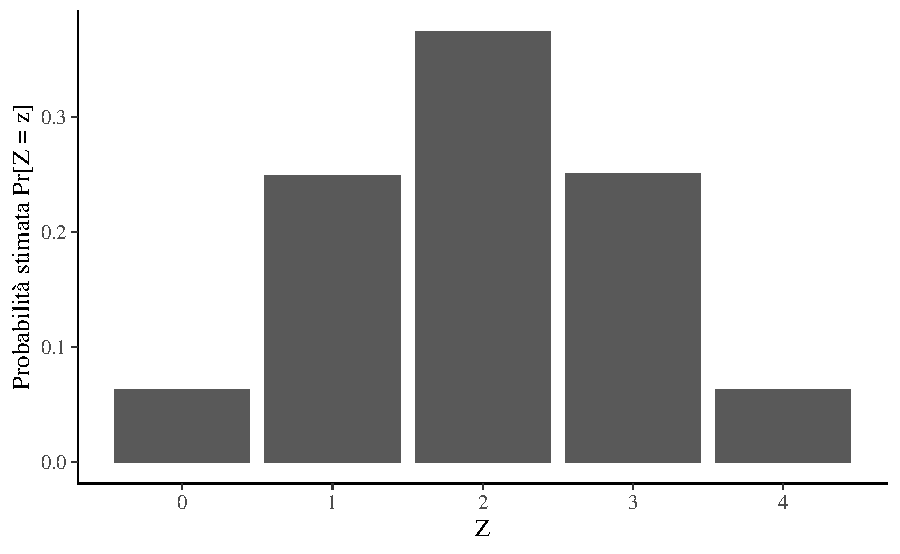
\includegraphics{ds4psy_files/figure-latex/barplot-mdf-4coins-1} 

}

\caption{Grafico di $M = 100\,000$ simulazioni della funzione di massa di probabilità di una variabile casuale definita come il numero di teste in quattro lanci di una moneta equilibrata.}\label{fig:barplot-mdf-4coins}
\end{figure}

Se \(A\) è un sottoinsieme della variabile casuale \(Z\), allora denotiamo con \(P_{z}(A)\) la probabilità assegnata ad \(A\) dalla distribuzione \(P_{z}\). Mediante una distribuzione di probabilità \(P_{z}\) è dunque possibile determinare la probabilità di ciascun sottoinsieme \(A \subset Z\) come

\[
P_{z}(A) = \sum_{z \in A} P_{z}(Z).
\]

\begin{example}
Nel caso dell'esempio discusso nella Sezione \ref{sec:fun-mass-prob}, la probabilità che la variabile casuale \(Z\) sia un numero dispari è \[
Pr(\text{Z è un numero dispari}) = P_{z}(Z = 1) + P_{z}(Z = 3) = \frac{4}{16} + \frac{4}{16} = \frac{1}{2}.
\]
\end{example}

\hypertarget{commenti-e-considerazioni-finali}{%
\section*{Commenti e considerazioni finali}\label{commenti-e-considerazioni-finali}}


In questo capitolo abbiamo visto come si costruisce lo spazio campionario di un esperimento casuale, quali sono le proprietà di base della probabilità e come si assegnano le probabilità agli eventi definiti sopra uno spazio campionario discreto. Abbiamo anche introdotto le nozioni di ``variabile casuale'', ovvero di una variabile che prende i suoi valori casualmente. E abbiamo descritto il modo di specificare la probabilità con cui sono presi i differenti valori, ovvero la funzione di distribuzione probabilistica \(F(X) = Pr(X < x)\), e la funzione di massa di probabilità. Le procedure di analisi dei dati psicologici che discuteremo in seguito faranno un grande uso di questi concetti e della notazione qui introdotta.

\hypertarget{regr-ml}{%
\chapter{Adattare il modello lineare ai dati}\label{regr-ml}}

\hypertarget{predictive-checks}{%
\chapter{Predictive checks}\label{predictive-checks}}

Nel Capitolo \ref{chapter-ppc} abbiamo visto come si genera la distribuzione predittiva a posteriori nel caso del modello più semplice: quello di un'unica variabile con una data distribuzione di probabilità. In questo capitolo estenderemo questa discussione al modello lineare. Esamineremo un esempio di \emph{posterior predictive check} in cui simuleremo da \(p(y^{rep} \mid \theta, y)\), usando le stime a posteriori dei parametri \(\theta\) del modello, e un esempio di \emph{prior predictive check} in cui simuleremo da \(p(y^{rep} \mid \mathcal{M})\), ovvero usando il meccanismo generatore dei dati del modello \(\mathcal{M}\) in esame, senza però includere i dati.

\hypertarget{campionamento-dalla-distribuzione-predittiva-a-posteriori}{%
\section{Campionamento dalla distribuzione predittiva a posteriori}\label{campionamento-dalla-distribuzione-predittiva-a-posteriori}}

La distribuzione predittiva a priori equivale alla distribuzione predittiva a posteriori, senza però i dati osservati. Quindi la distribuzione predittiva a priori non è altro che il caso limite della distribuzione predittiva a posteriori, calcolata però senza utilizzare i dati del campione. Il manuale Stan afferma che, se il codice per il il controllo predittivo a posteriori è già stato scritto, ed è possibile impostare il codice in modo che non sia necessario specificare i dati, allora non è necessario fare nient'altro.

Consideriamo qui un esempio nel quale vengono usati i dati \texttt{kidiq} \citep{gelman2020regression}.

\begin{Shaded}
\begin{Highlighting}[]
\FunctionTok{library}\NormalTok{(}\StringTok{"rio"}\NormalTok{)}
\NormalTok{df }\OtherTok{\textless{}{-}}\NormalTok{ rio}\SpecialCharTok{::}\FunctionTok{import}\NormalTok{(}\FunctionTok{here}\NormalTok{(}\StringTok{"data"}\NormalTok{, }\StringTok{"kidiq.dta"}\NormalTok{))}
\end{Highlighting}
\end{Shaded}

Iniziamo a generare un istogramma dei valori \(y\) stanardizzati:

\begin{Shaded}
\begin{Highlighting}[]
\NormalTok{df }\SpecialCharTok{\%\textgreater{}\%} 
  \FunctionTok{ggplot}\NormalTok{(}\FunctionTok{aes}\NormalTok{(}\FunctionTok{scale}\NormalTok{(kid\_score)[, }\DecValTok{1}\NormalTok{])) }\SpecialCharTok{+}
  \FunctionTok{geom\_histogram}\NormalTok{()}
\end{Highlighting}
\end{Shaded}

\begin{center}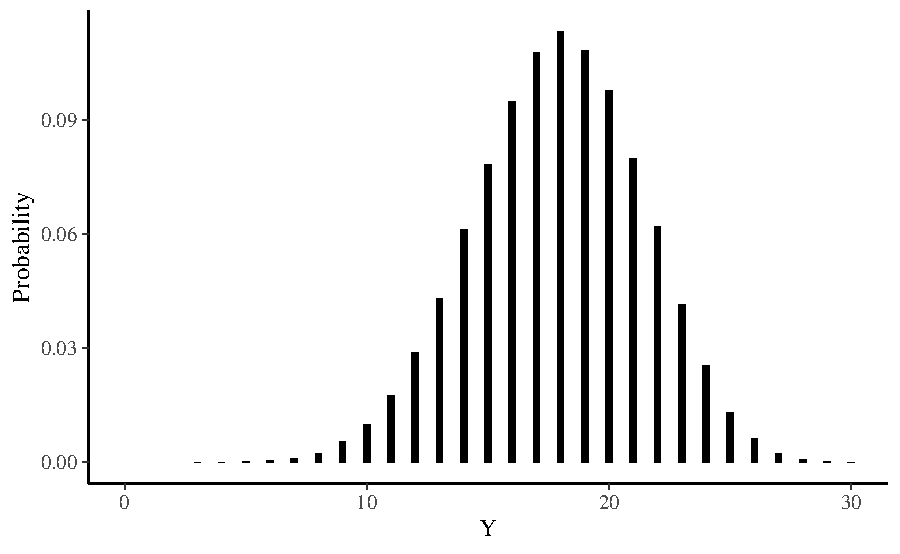
\includegraphics{ds4psy_files/figure-latex/unnamed-chunk-17-1} \end{center}

Per svolgere l'analisi bayesiana sistemiamo i dati (standardizzati) nel formato appropriato per Stan:

\begin{Shaded}
\begin{Highlighting}[]
\NormalTok{data\_list }\OtherTok{\textless{}{-}} \FunctionTok{list}\NormalTok{(}
  \AttributeTok{N =} \FunctionTok{length}\NormalTok{(df}\SpecialCharTok{$}\NormalTok{kid\_score),}
  \AttributeTok{x =} \FunctionTok{scale}\NormalTok{(df}\SpecialCharTok{$}\NormalTok{mom\_iq)[, }\DecValTok{1}\NormalTok{],}
  \AttributeTok{y =} \FunctionTok{scale}\NormalTok{(df}\SpecialCharTok{$}\NormalTok{kid\_score)[, }\DecValTok{1}\NormalTok{]}
\NormalTok{)}
\end{Highlighting}
\end{Shaded}

Il seguente listato specifica il codice Stan necessario per simulare dati dalla distribuzione predittiva a posteriori.

\begin{Shaded}
\begin{Highlighting}[]
\NormalTok{stancode }\OtherTok{\textless{}{-}} \StringTok{\textquotesingle{}}
\StringTok{data \{}
\StringTok{  int\textless{}lower=0\textgreater{} N;  }
\StringTok{  vector[N] x; }
\StringTok{  vector[N] y; }
\StringTok{\}}
\StringTok{parameters \{}
\StringTok{  real alpha;}
\StringTok{  real beta;}
\StringTok{  real\textless{}lower=0\textgreater{} sigma;}
\StringTok{\}}
\StringTok{model \{}
\StringTok{  alpha \textasciitilde{} normal(0, 1);}
\StringTok{  beta \textasciitilde{} normal(0, 1);}
\StringTok{  sigma \textasciitilde{} normal(0, 1);}
\StringTok{  y \textasciitilde{} normal(alpha + beta * x, sigma);}
\StringTok{\}}
\StringTok{generated quantities \{}
\StringTok{  vector[N] y\_rep;}
\StringTok{  for(i in 1:N)\{}
\StringTok{    y\_rep[i] = normal\_rng(alpha + beta * x[i], sigma);}
\StringTok{  \}}
\StringTok{\}}
\StringTok{\textquotesingle{}}
\FunctionTok{writeLines}\NormalTok{(stancode, }\AttributeTok{con =} \StringTok{"code/post\_pred\_check\_1.stan"}\NormalTok{)}
\end{Highlighting}
\end{Shaded}

\begin{Shaded}
\begin{Highlighting}[]
\NormalTok{file }\OtherTok{\textless{}{-}} \FunctionTok{file.path}\NormalTok{(}\StringTok{"code"}\NormalTok{, }\StringTok{"post\_pred\_check\_1.stan"}\NormalTok{)}
\NormalTok{mod }\OtherTok{\textless{}{-}} \FunctionTok{cmdstan\_model}\NormalTok{(file)}
\end{Highlighting}
\end{Shaded}

\begin{Shaded}
\begin{Highlighting}[]
\NormalTok{fit }\OtherTok{\textless{}{-}}\NormalTok{ mod}\SpecialCharTok{$}\FunctionTok{sample}\NormalTok{(}
  \AttributeTok{data =}\NormalTok{ data\_list,}
  \AttributeTok{iter\_sampling =}\NormalTok{ 4000L,}
  \AttributeTok{iter\_warmup =}\NormalTok{ 2000L,}
  \AttributeTok{seed =}\NormalTok{ SEED,}
  \AttributeTok{chains =}\NormalTok{ 4L,}
  \AttributeTok{parallel\_chains =}\NormalTok{ 2L,}
  \AttributeTok{refresh =} \DecValTok{0}\NormalTok{,}
  \AttributeTok{thin =} \DecValTok{1}
\NormalTok{)}
\end{Highlighting}
\end{Shaded}

\begin{Shaded}
\begin{Highlighting}[]
\NormalTok{stanfit1 }\OtherTok{\textless{}{-}}\NormalTok{ rstan}\SpecialCharTok{::}\FunctionTok{read\_stan\_csv}\NormalTok{(fit}\SpecialCharTok{$}\FunctionTok{output\_files}\NormalTok{())}
\end{Highlighting}
\end{Shaded}

Un istogramme dei valori \(y^{rep}\) può essere generato nel modo seguente:

\begin{Shaded}
\begin{Highlighting}[]
\FunctionTok{hist}\NormalTok{(}\FunctionTok{as.matrix}\NormalTok{(stanfit1, }\AttributeTok{pars =} \StringTok{"y\_rep"}\NormalTok{), }\AttributeTok{breaks =} \DecValTok{100}\NormalTok{)}
\end{Highlighting}
\end{Shaded}

\begin{center}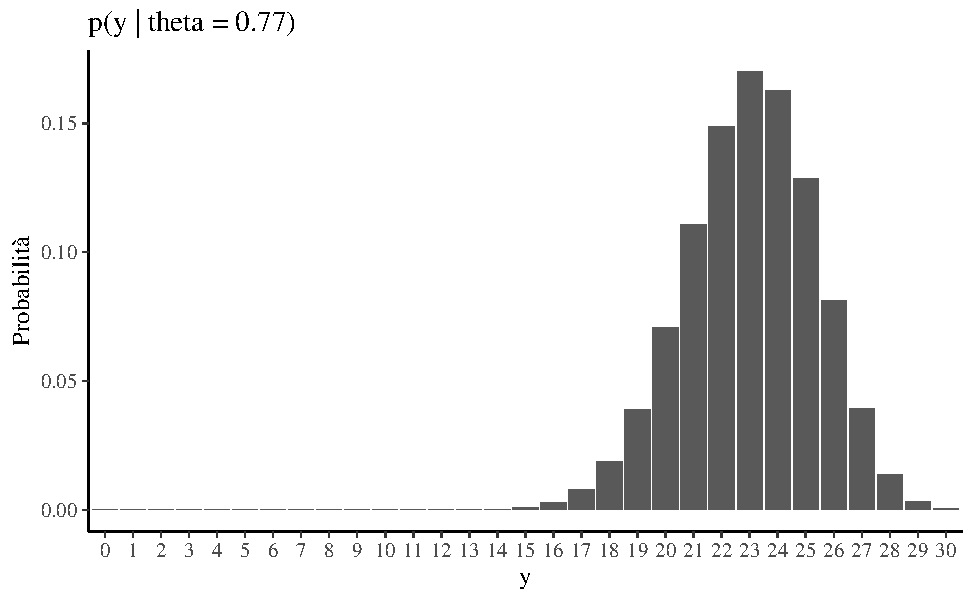
\includegraphics{ds4psy_files/figure-latex/unnamed-chunk-23-1} \end{center}

\hypertarget{campionamento-dalla-distribuzione-predittiva-a-priori}{%
\section{Campionamento dalla distribuzione predittiva a priori}\label{campionamento-dalla-distribuzione-predittiva-a-priori}}

Per comprendere le assunzioni che abbiamo introdotto nel modello, possiamo generare dati mediante il modello; tali dati, che sono generati interamente dalle distribuzioni a priori, sono chiamati distribuzione predittiva a priori. La generazione della distribuzione predittiva a priori ci aiuta a verificare se le distribuzioni a priori per i parametri del modello hanno senso. Quello che vogliamo sapere qui è: le distribuzioni a priori che abbiamo scelto generano dati che hanno caratteristiche realistiche?

Dal punto di vista della programmazione, l'unico cambiamento necessario rispetto al codice utilizzato per la distribuzione predittiva a posteriori è quello di eliminare la porzione di codice che fa riferimento ai dati \(y\) -- nel caso di un modello lineare, i valori \(x\) devono invece essere mantenuti per potere generare \(y^{sim}\) (nel codice questa variabile è ancora chiamata \texttt{y\_rep}).

\begin{Shaded}
\begin{Highlighting}[]
\NormalTok{data\_list }\OtherTok{\textless{}{-}} \FunctionTok{list}\NormalTok{(}
  \AttributeTok{N =} \FunctionTok{length}\NormalTok{(df}\SpecialCharTok{$}\NormalTok{kid\_score),}
  \AttributeTok{x =} \FunctionTok{scale}\NormalTok{(df}\SpecialCharTok{$}\NormalTok{mom\_iq)[, }\DecValTok{1}\NormalTok{]}
\NormalTok{)}
\end{Highlighting}
\end{Shaded}

\begin{Shaded}
\begin{Highlighting}[]
\NormalTok{stancode }\OtherTok{\textless{}{-}} \StringTok{\textquotesingle{}}
\StringTok{data \{}
\StringTok{  int\textless{}lower=0\textgreater{} N;  }
\StringTok{  vector[N] x; }
\StringTok{\}}
\StringTok{parameters \{}
\StringTok{  real alpha;}
\StringTok{  real beta;}
\StringTok{  real\textless{}lower=0\textgreater{} sigma;}
\StringTok{\}}
\StringTok{model \{}
\StringTok{  alpha \textasciitilde{} normal(0, 1);}
\StringTok{  beta \textasciitilde{} normal(0, 1);}
\StringTok{  sigma \textasciitilde{} normal(0, 1);}
\StringTok{\}}
\StringTok{generated quantities \{}
\StringTok{  vector[N] y\_rep;}
\StringTok{  for(i in 1:N)\{}
\StringTok{    y\_rep[i] = normal\_rng(alpha + beta * x[i], sigma);}
\StringTok{  \}}
\StringTok{\}}
\StringTok{\textquotesingle{}}
\FunctionTok{writeLines}\NormalTok{(stancode, }\AttributeTok{con =} \StringTok{"code/prior\_pred\_check\_1.stan"}\NormalTok{)}
\end{Highlighting}
\end{Shaded}

\begin{Shaded}
\begin{Highlighting}[]
\NormalTok{file }\OtherTok{\textless{}{-}} \FunctionTok{file.path}\NormalTok{(}\StringTok{"code"}\NormalTok{, }\StringTok{"prior\_pred\_check\_1.stan"}\NormalTok{)}
\NormalTok{mod }\OtherTok{\textless{}{-}} \FunctionTok{cmdstan\_model}\NormalTok{(file)}
\end{Highlighting}
\end{Shaded}

\begin{Shaded}
\begin{Highlighting}[]
\NormalTok{fit }\OtherTok{\textless{}{-}}\NormalTok{ mod}\SpecialCharTok{$}\FunctionTok{sample}\NormalTok{(}
  \AttributeTok{data =}\NormalTok{ data\_list,}
  \AttributeTok{iter\_sampling =}\NormalTok{ 4000L,}
  \AttributeTok{iter\_warmup =}\NormalTok{ 2000L,}
  \AttributeTok{seed =}\NormalTok{ SEED,}
  \AttributeTok{chains =}\NormalTok{ 4L,}
  \AttributeTok{parallel\_chains =}\NormalTok{ 2L,}
  \AttributeTok{refresh =} \DecValTok{0}\NormalTok{,}
  \AttributeTok{thin =} \DecValTok{1}
\NormalTok{)}
\end{Highlighting}
\end{Shaded}

\begin{Shaded}
\begin{Highlighting}[]
\NormalTok{stanfit2 }\OtherTok{\textless{}{-}}\NormalTok{ rstan}\SpecialCharTok{::}\FunctionTok{read\_stan\_csv}\NormalTok{(fit}\SpecialCharTok{$}\FunctionTok{output\_files}\NormalTok{())}
\end{Highlighting}
\end{Shaded}

Questo è un istogramma della distribuzione preditiva a priori. Tale distribuzione viene usata per valutare se le distribuzioni a priori dei parametri sono sensate. Concludiamo che sono sensate se la distribuzione preditiva a priori include tutti i valori possibili della distribuzione della \(y\), senza scostarsti troppo da essa.

\begin{Shaded}
\begin{Highlighting}[]
\FunctionTok{hist}\NormalTok{(}\FunctionTok{as.matrix}\NormalTok{(stanfit2, }\AttributeTok{pars =} \StringTok{"y\_rep"}\NormalTok{), }\AttributeTok{breaks =} \DecValTok{100}\NormalTok{)}
\end{Highlighting}
\end{Shaded}

\begin{center}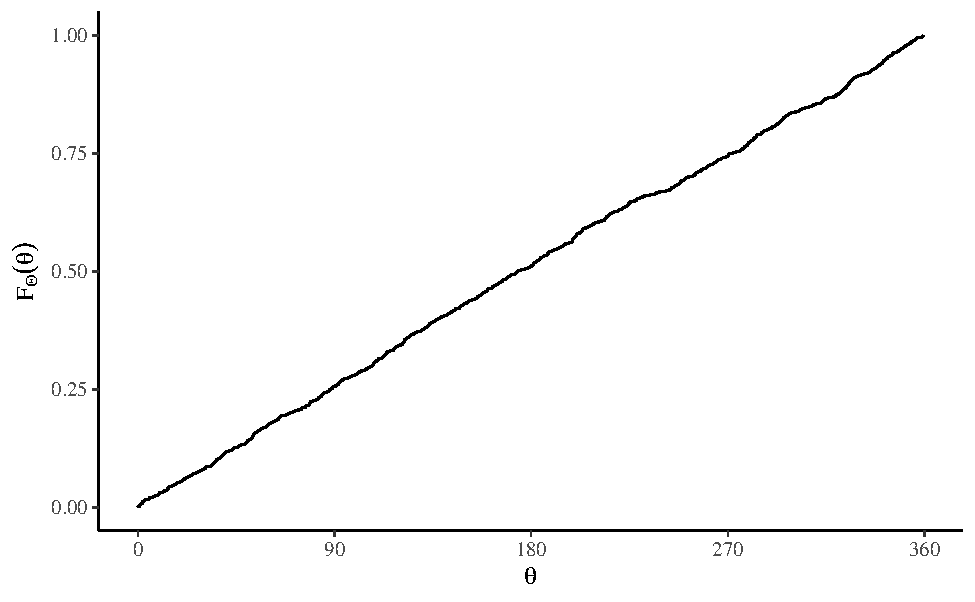
\includegraphics{ds4psy_files/figure-latex/unnamed-chunk-29-1} \end{center}

\hypertarget{commenti-e-considerazioni-finali-1}{%
\section*{Commenti e considerazioni finali}\label{commenti-e-considerazioni-finali-1}}


I due \emph{predictive checks} che abbiamo esaminato in questo capitolo servono due scopi diversi.

La distribuzione predittiva a priori viene utilizzata per comprendere le assunzioni introdotte nel modello. Per fare questo possiamo generare dei dati dal modello. Tali dati, che vengono prodotti interamente dalle distribuzioni a priori, sono chiamati distribuzione predittiva a priori. La distribuzione predittiva a priori ci aiuta a capire se le distribuzioni a priori per i parametri del modello hanno un senso. Quello che ci chiedimo è: le distribuzioni a priori generano dei dati che hanno caratteristiche realistiche? Una risposta affermativa a tale domanda corrisponde ad una distribuzione predittiva a priori che è più ampia della distribuzione dei dati osservati, in linea con il principio dei prior debolmente informativi. Tale distribuzione dovrebbe avere almeno una qualche massa nell'intorno ai valori estremi, ma plausibili dei dati; non dovrebbe, invece, esserci massa in corrispondenza di valori di dati completamente implausibili.

La distribuzione predittiva a posteriori viene invece utilizzata per esplorare le caratteristiche che potrebbero avere i possibili dati futuri. L'idea alla base del controllo predittivo a posteriori è semplice: se un modello è appropriato, dovremmo essere in grado di usarlo per generare dati che assomigliano ai dati che abbiamo osservato nel campione. La motivazione è simile a quella che ci ha condotto alla distribuzione predittiva a priori, tranne per il fatto che ora abbiamo un modello generativo dei dati basato sui dati osservati.

  \bibliography{refs.bib,book.bib,packages.bib}

\printindex

\end{document}
